\documentclass[11pt,a4paper]{article}

% Paper five, the flagship: Finitely Verifiable Segmentation. Drafted from the skeleton note
% (notes/paper-five-skeleton.md) under the approved framing: the definition is presented as the
% organizing hypothesis whose consequences are the contribution, not as a claimed-new notion, until
% the primary reads settle novelty; the empirical material appears as brief instances deferring to
% the two companion papers; related work is written from the completed primary reads. Every stated result names its
% machine-check module in a comment, and no section may claim what its named derivation does not
% hold; the quoted counts are the modules' own output lines, re-derivable by run-all.sh and held by
% scripts/check-paper5.sh.

\usepackage[margin=1in]{geometry}
\usepackage{amsmath}
\usepackage{amssymb}
\usepackage{amsthm}
\usepackage{array}
\usepackage{booktabs}
\newcolumntype{L}[1]{>{\raggedright\arraybackslash}p{#1}}
\usepackage{tikz}
\usepackage[numbers]{natbib}
\usepackage{needspace}
\usepackage[hidelinks,unicode]{hyperref}
% The build writes source-digest.tex with the digest of these sources (scripts/build-paper.sh); the document carries
% it in its Keywords so the gate can hold the shipped pdf to the sources beside it. A build without the file says so.
\InputIfFileExists{source-digest.tex}{}{\newcommand{\SourceDigest}{unrecorded}}
\hypersetup{
  pdftitle={Finitely Verifiable Segmentation: Decidability for Every Tokenizer with a Finite-State Verifier},
  pdfauthor={Nicklas Nidhögg},
  pdfsubject={Segmentation policies; finite verifiers; decidability; rational relations},
  pdfkeywords={segmentation, tokenization, finite verifier, decidability, rational relations, source-sha256:\SourceDigest}
}
\widowpenalty=10000
\clubpenalty=10000

\theoremstyle{definition}
\newtheorem{definition}{Definition}

\theoremstyle{plain}
\newtheorem{theorem}{Theorem}
\newtheorem{lemma}{Lemma}
\newtheorem{corollary}{Corollary}
\newtheorem{proposition}{Proposition}

\newcommand{\code}[1]{\texttt{#1}}

% The default itemize bullet pulls in a Type 3 bitmap font, which some submission systems reject. The math bullet
% comes from the Type 1 symbol font that is embedded already.
\renewcommand{\labelitemi}{\(\bullet\)}

\title{Finitely Verifiable Segmentation:\\Decidability for Every Tokenizer with a Finite-State Verifier}
\author{Nicklas Nidh\"ogg\\[0.4em] \normalsize Independent Researcher\\ \normalsize
\texttt{nicklas.nidhogg@gmail.com}\\ \normalsize ORCID: 0009-0006-6161-6150}
\date{October 16, 2026}

\begin{document}
\maketitle

\begin{abstract}
A segmentation policy assigns to each byte string at most one segmentation into tokens. Call it
\emph{finitely verifiable} when a finite automaton over marked strings, bytes paired with boundary bits, accepts exactly
the policy's own segmentations. The automaton judges a proposed segmentation and need not compute one. From a supplied
verifier the paper gives constructive decisions for four questions, whether a window certifies a token boundary, whether
the boundary gap is bounded, whether a mask can keep generation from dead-ending, and whether two policies are
equivalent. The last three specialize limitedness, co-accessibility and the equivalence of single-valued transducers.
The first refines the synchronizing cut of code theory, and two more ask whether a certified cut, or the cuts of an
inventory, let each piece scan alone. The class sits strictly between the online-scannable policies and those with
regular domains, and its inner frontier is Choffrut's and decidable in polynomial time. Markings are length-preserving,
so the class is exactly the rational segmentation policies, a normal form rather than a restriction. The class is closed
under four pipeline operations, composition over a labeled stage, restriction to a regular schema, splitting at
character-class changes, and byte-fallback union of literal policies. Each composite inherits the six decisions, and
certificates transfer between stages under four laws. Under rational, unifilar, almost surely stopping finite-state
sources, each mass of the weighted section is an exact rational, and so is each rate where expected length is positive.
Maximal-munch lexing, canonical byte-pair encoding and two-mode WordPiece instantiate the interface, and the munch
library implements all six decisions. Every theorem carries an executable check, and every reported statistic is a
program's own output.
\end{abstract}

\section{Introduction}

A production system may need to know where its byte stream resynchronizes after a lost fragment, how far that stream can
run before a token boundary is guaranteed, whether a grammar-masked generator can be left with no admissible next token,
and what a tokenizer upgrade does to cached segmentations. Exact procedures answer some of these in particular settings,
such as masks in constrained decoding~\citep{koo2024automata} and the equivalence of byte-pair
dictionaries~\citep{berglund2024bpedfa}. Each question quantifies over all inputs, and a finite sample of inputs cannot
establish such a universal guarantee. From a supplied verifier, this paper gives constructive decisions for all four,
certification, the boundary gap, realizability and equivalence.

The series began with certified bytes~\citep{nidhogg2026splitpoints} and certified
windows~\citep{nidhogg2026splitwindows} for maximal-munch scanning, and its two companion studies answered special cases
of those questions. The recovery companion \citep{nidhogg2026panic} proved that certificates make resuming after damage
sound. The splitting companion \citep{nidhogg2026splitting} read the same certificates forward into speculation-free
work division, and decided certification, the anchor-free span, and segmentation differentials for regular token sets.
The present paper states what those decisions were always instances of. It rests on one hypothesis.

% The definition is the paper's object and is kept on one page.
\Needspace{7\baselineskip}
\begin{definition}[Segmentation policy; finite verifiability]\label{def:fv}
A \emph{segmentation policy} assigns to each string at most one segmentation, none when the string is not tokenizable. A
segmentation here is an unlabeled partition of the string into consecutive nonempty pieces, equivalently its boundary
bit pattern, the boundary projection of what the splitting companion calls a segmentation. The names a stage gives those
pieces are separate labeler data, which is why two policies naming identical spans differently are the same policy. A
\emph{marked string} pairs each byte with one bit, whether a token boundary follows that byte's position, and a position
$i$ of it is a \emph{token start} exactly when $i = 0$ or the bit at $i-1$ is set. A policy is
\emph{finitely verifiable} when some deterministic finite automaton over marked strings accepts exactly the markings
that are the policy's own segmentations of its tokenizable strings.
\end{definition}

The verifier decides a \emph{proposed} segmentation by reading it. It need not compute the segmentation online, and that
distinction is the crux of the paper. Section~\ref{sec:real} exhibits a policy with no finite-state bounded-delay
scanner that is nevertheless finitely verifiable. Verification is the strictly weaker demand, and everything below asks
only for it.

The class is not new, and the paper does not present it as new. A finitely verifiable policy is a length-preserving
partial \emph{automatic function} in the sense of \citet{case2013automatic}, its graph a functional synchronous
relation, regular under convolution. The text keeps the verifier-first name because the verifier is the interface every
construction below programs against. Section~\ref{sec:related} surveys the transducer literature. The first three
contributions below were not found in it and are what the paper claims as its own; the last two place the class and
carry it to real tokenizers.

The contributions are:

\begin{itemize}
\item The four decisions, and the two that ask whether certified cuts let the pieces scan alone, run on supplied
verifier presentations with constructive outputs and survive the four pipeline operations of Theorem~\ref{thm:calculus},
composition over a labeled stage, restriction to a regular schema, splitting at character-class changes and
byte-fallback union of literal policies (Sections~\ref{sec:four} and~\ref{sec:calculus}).
\item Certificates transfer between stages under proved laws, with an exact stage-local lift
(Section~\ref{sec:transfer}).
\item Zero differential mass is identified with the absence of a boundary differential in the source's support, and the
exact masses behind it are solved from the supplied verifiers through the same interface (Section~\ref{sec:weighted}).
\item The class sits strictly between the online-scannable policies and those with regular domains, its inner frontier
is decidable in polynomial time, and over the marking encoding it is exactly the rational segmentation policies
(Section~\ref{sec:real}).
\item Literal and regular maximal munch, canonical byte-pair encoding and two-mode WordPiece carry the interface, each
validated against an independent reference scanner or encoder, and the munch library implements all six decisions
(Sections~\ref{sec:interface} and~\ref{sec:instances}).
\end{itemize}

\begin{table}[tp]
\centering \small
\begin{tabular}{L{2.8cm}L{8.0cm}L{3.8cm}}
\toprule Result & Statement & Where \\ \midrule Four decisions & Certification, the boundary gap and realizability are
decidable for every supplied verifier, and full equivalence for every pair of them; certification returns a counterexample when negative, equivalence a differing string, the boundary gap a pumpable lasso, and realizability the mask & Theorem~\ref{thm:four} \\
\addlinespace Cut and chunk independence & Whether a certified cut lets both its sides scan alone, and whether all of an
inventory's cuts do at once, are decidable, each with a shortest counterexample; the first for every pair implies the
second, not conversely; every maximal-munch cut and inventory is independent, WordPiece and threshold-splice ones need
not be & Theorems~\ref{thm:cut} and~\ref{thm:chunk} \\ \addlinespace Where the class sits & A regular token set with
unbounded commit delay has no finite-state scanner yet a finite verifier; non-regular domains are outside; a regular
domain is not sufficient & Section~\ref{sec:real}, Lemma~\ref{lem:outside}, Proposition~\ref{prop:regular-domain} \\
\addlinespace A normal form & Markings are length-preserving, so finite verifiability coincides with rationality of the
marking relation; undecidability sits in presentations that do not convert effectively to a verifier & Proposition~\ref{prop:collapse}, Section~\ref{sec:real} \\ \addlinespace Closure & Pipelines over a labeled stage one,
restrictions, splitter pre-tokenizers and byte-fallback unions of literal policies stay in the class and inherit all six
decisions & Theorem~\ref{thm:calculus} \\ \addlinespace Transfer & Certificates are monotone under restriction, forced
at splitter boundaries, subset-bounded through pipelines, and lifted through pipelines exactly when a product of two
stage-local automata is empty, with a per-label side condition as the sufficient corollary; a tower's certificate
factors through its levels on the tower's own domain & Propositions~\ref{prop:monotone} to~\ref{prop:subset},
Theorem~\ref{thm:lift}, Corollary~\ref{cor:labels}, Proposition~\ref{prop:stack} \\ \addlinespace Weighted theory &
Under rational, unifilar, almost surely stopping sources the tokenizability and differential masses of
Section~\ref{sec:weighted} are exact rationals, as are the unnormalized expected length and expected token, mismatch and
boundary counts, and every rate whose expected length is positive; and differential mass is nonzero exactly when a
boundary differential lies in the source's support & Theorem~\ref{thm:weighted}, Proposition~\ref{prop:positivity} \\
\addlinespace Instances & Literal maximal munch, regular-token maximal munch, canonical byte-pair encoding and two-mode
WordPiece carry the whole interface, each validated against an independent reference scanner or encoder; under maximal
munch a certified window makes a cache keyed on its cut sound for continuations that keep the window and that the policy
tokenizes completely & Section~\ref{sec:interface}, Proposition~\ref{prop:cache} \\ \bottomrule
\end{tabular}
\caption{What the hypothesis of Definition~\ref{def:fv} buys, and where each result is stated and proved. Each
computation behind a row has an executable check, named in a source comment in its section or held by the claims gate;
the outside lemma and the collapse proposition are proofs alone.} \label{tab:results}
\end{table}

Table~\ref{tab:results} summarizes the results and names the statements that carry them. Three points of scope hold
throughout and are stated here once. First, the theorems assume a \emph{supplied} verifier, presented as its states,
transitions, acceptance and alphabet. A mere promise that some program computes a policy in the class is not enough,
since the reductions of Section~\ref{sec:real} leave the four questions without a uniform procedure. Second, membership
in the class is determined by the marking relation, whatever its presentation. A policy whose domain is not regular lies
outside the class, but a regular domain alone does not put it inside. Third, every validation sweep is bounded, in that
it checks every case within its declared universe and says nothing beyond it, so a sweep supports a theorem but never
replaces its proof.

\section{The definition and the interface}\label{sec:interface}

% machine-check: finitely_verifiable.py (literal policy: 1,530 strings across 6 token sets;
% regular policy: 381 strings across 3 regex sets including the set with no online scanner;
% wordpiece policy: 765 strings across 3 two-mode pairs; every marking of every string tried,
% the verifier's accepted markings exactly the reference scan's in each case).

The whole paper programs against four methods, \code{start}, \code{step(state, byte, mark)} returning a successor state
or refusal, \code{accepts(state)}, and \code{alphabet}. An object with those four methods is a policy the theorems cover
when it presents a \emph{finite, effective} verifier, which means finitely many reachable states and a finite alphabet,
both enumerated once per decision. The executable modules take the alphabet's symbols as one-character strings, and
windows and the strings a decision returns are spelled over them. The verifier's accepted language must be
\emph{functional}, at most one accepted marking per byte string, and \emph{well formed}, every nonempty accepted marking
ending in a zero bit, the final-zero convention, so that it encodes a segmentation. A byte outside an object's own
alphabet leaves its domain by definition, and every decision treats that side as dead without stepping its verifier, so
the interface requires no behavior of a verifier on a foreign byte. Functionality can also be checked at the interface.
The self-product that guesses two markings of one byte stream and latches their first disagreement is empty exactly when
the object is functional. The other half of being a policy is that every nonempty accepted marking closes with a zero
bit, which is read off the transitions into accepting states. Nothing below inspects a policy's internals.

A marked string is best read as a scan's transcript. Take the token set $\{\code{ab}, \code{b}\}$ under maximal munch
and the input \code{bab}. Its unique segmentation is $\code{b} \cdot \code{ab}$, and its marked string pairs the bytes
\code{b}, \code{a}, \code{b} with the boundary bits $1, 0, 0$, one bit per byte saying whether a token boundary follows
that byte, so a set bit closes the current token and the next one begins at the following byte. The bit after the final
byte is always zero, since the string's end closes the last token and a boundary there would open an empty segment. The
verifier for this policy accepts exactly the marked strings whose bits close segments that are tokens and never close
one while a strictly longer token could still complete, and it accepts nothing at all for an input like \code{ba}, which
no segmentation covers. The splitting companion's armed-run verifier carries the same information on the other side of
each byte, a mark on every token start, position zero included, so its mark at position $i+1$ is the bit here at
position $i$. A one-byte buffer translates either encoding into the other, so finite verifiability does not depend on
the choice. Everything the paper does is a question about the regular language of such transcripts.

Two conventions about the empty input are fixed here because later constructions lean on them. First, the empty input
carries no bits and admits one candidate segmentation, the empty sequence, but whether that segmentation is in a
policy's domain varies. The three maximal-munch tokenizers below consume the empty input trivially and accept it. A
policy accepting nothing does not, and neither does a restriction to a schema that excludes the empty input. The
presentation-level reductions of Section~\ref{sec:real} need policies of exactly that kind. The verifier answers that
question from its own start state, and it must, since Lemma~\ref{lem:outside} reads the policy's domain off the
projection of the accepted language, and that reading is right only if the automaton, and no fact recorded beside it,
decides the empty input. Second, the start state is kept distinct from every configuration reachable after a byte, which
any start state no step re-enters provides. The point is that whether nothing has been consumed is a fact about the run,
which a configuration alone does not record. A derivative automaton for $\code{a}(\code{aa})^{*}$ returns to its initial
configuration after \code{aa}, and reading the return as an unconsumed state accepts two markings of that string. Under
the normalization the start state's acceptance is exactly the empty input's membership, and every product and
enumeration below uses it.

Three policies whose scanners share no code carry the interface, as a test of its generality. For literal maximal munch,
a verifier run pairs a candidate token with the length consumed so far. At the next proposed mark the segment the run
spans must be accepted by some token, and from then on the run is armed. A run that completes a token while armed has
found a longer match past a commit, which greedy scanning forbids. For regular-token maximal munch, the runs are
Brzozowski derivatives of the token expressions, armed the same way, and the tested sets include $\{a^{+}b,\ a\}$, which
no online scanner decides. For two-mode WordPiece, the verifier carries the mode bit, and a closed segment flips it to
continuation, which is the split of subword tokenizers between word-initial and mid-word vocabularies. Each verifier is
validated against an independent reference scanner, namely the direct greedy scan, a longest-language-match reference
over regular expressions, and the two-mode scan respectively, on every marking of every string of bounded length. In
each case the verifier accepts exactly the reference segmentation of each tokenizable string and nothing for the
untokenizable ones, over 1{,}530, 381, and 765 strings.

\section{The four decisions}\label{sec:four}

% machine-check: finitely_verifiable.py (generic certification equal to the specialized product
% decider on 36 triples, refutations re-verified against the scan; generic equivalence equal to
% the specialized armed-run product on 9 regex pairs with differing strings re-verified, plus one
% cross-representation pair; generic boundary gap equal to the known literal gaps and the
% unbounded verdict on the unbounded-delay set, and separated from the anchor-free span over
% {aa, a}, where the supremum is the longest token and every window is refuted; generic
% realizability fixpoint-clean on one policy of each kind).

Four questions are decidable, three for every supplied verifier and equivalence for every pair of them, with the
counterexamples and constructive outputs stated below. The theorem states them and the proof gives one finite
construction per question. As the introduction states, the theorem's hypothesis is a given presentation, which mere
membership in the class does not supply. One phrase is fixed first, since the first decision and every transfer law of
Section~\ref{sec:transfer} use it.

\begin{definition}[Correct covering; certification]\label{def:cover} For a window $W$ of length $h$ and an origin
$0 \le o < h$, a policy $P$ \emph{covers} an occurrence of $W$ at position $p$ of a string in its domain
\emph{correctly} when $p+o$ is a token start of $P$'s segmentation and no token start lies in $(p+o,\,p+h-1]$.
Equivalently, the token covering the occurrence's final byte begins exactly $o$ bytes into it. $P$ \emph{certifies}
$(W,o)$ when it covers every occurrence of $W$ in every string of its domain correctly.
\end{definition}

\begin{theorem}[The four decisions]\label{thm:four} Let a well-formed functional finite verifier presenting a
segmentation policy be given as its states, its transition and acceptance functions, and its finite alphabet. The
following are decidable, uniformly in the verifiers given, and each answer comes with the object named.
\begin{enumerate}
\item \textbf{Certification.} Given a nonempty window $W$ and an origin $0 \le o < |W|$, whether the policy certifies
$(W,o)$; when it does not, a string of the domain with an occurrence it covers wrongly.
\item \textbf{Boundary gap.} Whether the length of a boundary-free stretch is bounded over the policy's segmentations;
when it is, the exact supremum, and when it is not, a pumpable lasso of the verifier.
\item \textbf{Realizability.} Whether the domain is nonempty; when it is, the mask that admits at each
\emph{completable} state, one from which an accepted completion exists, exactly the steps after which an accepted
completion remains, under which generation from any completable state never dead-ends.
\item \textbf{Equivalence.} Given two such verifiers, whether the two policies have the same domain and the same
segmentation on it, and separately each half of that: whether they segment every string of their common domain alike,
and whether their domains are equal. Each failure comes with a differing string, one in one domain and not the other or
one in both domains segmented apart.
\end{enumerate}
\end{theorem}

Three remarks fix the statement's terms. Throughout, \emph{boundary gap} names the stretch of the second item, between
consecutive token boundaries, and its supremum. The leading stretch, from position zero to the first boundary, and the
trailing stretch, from the last boundary to the end of the input, count the same way, end of input being an implicit
close, and a string with no marked boundary is one stretch entire. A domain that is empty or holds the empty string
alone has no stretch, and its supremum is zero by convention, a value the decision returns although no stretch attains
it. Realizability guarantees that generation never blocks, and it says nothing about whether a run stops. An empty
domain answers no, and on a nonempty one the computed mask is the positive answer's output. The supplied verifier is
needed even for the boundary gap's yes-or-no, which Proposition~\ref{prop:gap-bounded} shows undecidable from a program
promised to compute a policy of the class.

% machine-check: the two decisions below are held by check-paper5.sh against the product decider
% and the equivalence instruments directly, so the worked example cannot drift from a run.
Two worked decisions fix the ideas at their smallest. Over $\{\code{ab}, \code{b}\}$, the window $(\code{b}, 0)$ is
\emph{refuted}, since the input \code{ab} is one token whose \code{b} sits mid-token, and the decision's counterexample
is that very string. The window $(\code{ab}, 0)$ is \emph{certified}, since \code{ab} occurs in tokens only
token-initially, so every occurrence in every tokenizable input begins a token. The two halves of the equivalence
decision separate cleanly on $\{\code{ab}, \code{b}\}$ against $\{\code{ab}, \code{b}, \code{a}\}$. Adding the one-byte
token creates a domain difference, the differing string \code{a}, tokenizable only on one side, while the boundary half
finds no \emph{boundary differential}, no commonly tokenizable string the two segment apart, because on every commonly
tokenizable string the added token never wins a longest match. The two policies are one segmenter on their common domain
and differ only in reach. Domain difference and boundary differential are independent findings, and the deciders
separate them with differing strings.

\begin{proof} One shape proves all four. The verifier is finite, and each property is decided by a finite computation
over the verifier or a product with it, namely reachability or emptiness for certification and equivalence, a cycle
search and a longest path for the boundary gap, and a co-accessibility mask for realizability. Each returned string is
read back from its search path. Throughout, functionality is used freely. A policy assigns at most one segmentation per
string, and the verifier accepts exactly the graph, so an accepted marking \emph{is} the policy's segmentation of its
byte projection.

\emph{Certification.} Fix the window $W$ with $h = |W|$ and origin $o$. In a marked string the token covering position
$j$ begins at the last token start at most $j$, which is why the two readings of Definition~\ref{def:cover} agree.
Correct covering of the occurrence at $p$ comes down to two facts about the $h$ token-start indicators of the
occurrence's positions. Build the product of the verifier with a matcher that nondeterministically designates one
occurrence of $W$ in the byte projection and records those bits as it passes. A state is violating when its designated
occurrence has completed with the covering condition false. The pair is refuted exactly when a violating state can
complete to acceptance, which is reachability in a finite graph, and the reachability path projects to a violating input
with its own segmentation as the exhibit.

\emph{Boundary gap.} Restrict the verifier to its live states, those reachable from the start and from which acceptance
is reachable, since only live states occur in accepted runs. Consider the subgraph of transitions whose mark bit is
zero. If it contains a cycle through a live state, pumping the cycle inside any accepting run through that state
produces accepted markings with arbitrarily long boundary-free stretches, so the boundary gap is unbounded. The output
is the lasso, a pumpable family, no single string exhibiting unboundedness. If it is acyclic, every boundary-free
stretch is scored off its zero-edge path with its closing byte counted where one exists. An internal stretch of $k$ zero
edges ends in a mark-one byte and spans $k+1$ bytes; a final stretch ends at accepting end of input and spans its $k$
zero edges alone, the terminal byte carrying the non-closing bit. The supremum is the larger of the two maxima over the
finite acyclic graph, computable and, wherever a stretch exists at all, attained. The empty and empty-string-only
domains take the conventional zero, which no stretch attains. Scoring the zero path alone would undercount every
internal stretch by its closing byte. The policy $\{\code{aab} \mapsto 010\}$ segments as $\code{aa}\,|\,\code{b}$ with
boundary gap two against a longest zero path of one.

\emph{Realizability.} Call a state completable, or co-accessible, when some marked suffix leads from it to an accepting
state. Completability is a reverse reachability fixpoint, computed once. The mask admits, at state $q$, exactly the
pairs $(\sigma, m)$ with $\code{step}(q, \sigma, m)$ completable. Suppose generation stands at a completable state $q$.
If $q$ accepts, generation may stop; if not, completability of $q$ names a marked suffix to acceptance, whose first step
the mask admits, so at least one admitted step exists and preserves completability. A masked generator therefore never
dead-ends, and the mask is computable from the fixpoint. The hypothesis that generation begins at a completable state is
needed, since a verifier accepting nothing is a policy of this class whose start state completes to nothing. Its mask
offers neither a stop nor a step, and the instrument refuses it, since a guarantee there would hold vacuously. Of the
four this is the shallow one, an implementation recipe once co-accessibility is computed, kept among the decisions
because the interface makes the guarantee available wherever the other three are.

\emph{Equivalence.} Three terms are fixed first and used in these senses throughout. Boundary equivalence is agreement
of the two segmentations on the common domain. A domain difference is a string tokenizable under exactly one policy.
Full equivalence is boundary equivalence together with the absence of any domain difference, and the item asks about it
first, the reductions of Section~\ref{sec:real} separating pairs on it with their differing strings on the domain half.

Full equivalence is language equality, and that is the first decision. Functionality gives a policy exactly one accepted
marking per string of its domain, so a verifier's accepted language is the policy's graph, the marked strings it accepts
being the pairs of a domain string and that string's own segmentation. Two policies are therefore fully equivalent
exactly when their accepted marked-string languages are equal. In one direction, equal languages have equal byte
projections, and those projections are the two domains. On a string both domains contain, the marking the first side
accepts lies in the second side's language too, and the second accepts exactly one marking of that string, so the two
segmentations agree there. In the other, unequal languages carry a marked string one side accepts and the other does
not, whose bytes either leave one domain or are segmented apart, and either way the policies are not fully equivalent.
Both verifiers are deterministic over the alphabet of (byte, bit) pairs, so this is equality of two deterministic
automata. Build the product over that alphabet, a byte outside one policy's own alphabet sending that side to a dead
state without its verifier being stepped, and search the product for a reachable pair in which exactly one side accepts.
Breadth-first search returns the shortest such marked string, or reports that no such pair is reachable. The search
visits each product state once, so the decision costs the product's size. Its states are the pairs of the two verifiers'
states with a dead state adjoined on each side, and out of each pair it has one edge per bit for every byte of the union
alphabet.

The two halves are decided separately, each by a product of its own, and the same products read a differing string for
the full decision. Which half a separation falls in is a further fact about it, the reductions of Section~\ref{sec:real}
separating on the domain half and the pipeline applications asking which half they have. Boundary equivalence is decided
by the first product. Run both verifiers over one byte stream with independently guessed marks $(m_1, m_2)$ and a flag
that latches when $m_1 \neq m_2$. A byte outside one policy's own alphabet is outside its domain, so no jointly accepted
stream contains one, and this product walks the intersection of the two alphabets. If a run reaches joint acceptance
with the flag set, functionality turns the two accepted markings into the two policies' own segmentations of the same
input, and they differ at the latched position, which gives a boundary differential with the input synthesized from the
path. Conversely a differential input yields such a run by guessing both true markings. Emptiness of flagged joint
acceptance is boundary equivalence.

Domain difference is the other half, and it needs a product of its own, since the first accepts only strings both
policies tokenize. That product walks the union of the two alphabets, the side whose alphabet lacks the byte recorded as
dead while the other runs on. Each policy's domain is the byte projection of its verifier's language, regular by
projection, so the difference of the two domains is regular and its emptiness decidable. The construction that yields a
differing string is the subset product. Track, for each side, the set of verifier states its surviving marking guesses
can occupy after the bytes read so far, which is that side's subset construction and finite. The string read so far is
in one side's domain exactly when some state in its set accepts, so a reachable pair of sets in which one side accepts
and the other does not marks a differing string, and the bytes labeling the path to it reconstruct the string.
Breadth-first search over pairs of subsets terminates and returns the shortest such string, or reports that the domains
coincide.
\end{proof}

% machine-check: segmentation_equivalence.py (literal product of two pending automata: 225 ordered pairs,
% boundary and domain verdicts equal to brute force on every pair, 60 differentials and 208 domain
% splits, differing strings re-verified; regular armed-run product: 25 ordered pairs, verdicts equal to
% brute force, 18 differing strings re-verified, the pool including sets whose online scanners do not
% exist; language-equality route: 251 pairs, both pools and the cross-representation pair, the one
% product equal to the two-half decision on every pair, 228 shortest differing strings re-verified).
The generic deciders are validated against the purpose-built ones they generalize. Certification is checked against the
pending-automaton product on 36 triples, and equivalence against the armed-run product on 9 regex pairs with every
differing string re-verified. The boundary gap is checked against the known literal boundary gaps, that is, each set's
longest token, and against the unbounded verdict on the unbounded-delay set, and realizability is fixpoint-clean on one
policy of each kind. One validation only the interface can express is that a literal policy and the regular policy
denoting the same token languages are proved equivalent across representations. For maximal munch the splitting
companion's two instruments, the product of two pending automata for literal policies and the armed-run product for
regular ones, are validated against brute force on 225 and 25 ordered pairs. The language-equality decision is held to
the two-half decision on all 251 pairs, the two pools together with the cross-representation pair. One product over
marked strings returns a differing string exactly where the two-half decision returns one, and each of the 228 shortest
differing strings is replayed against the reference scans, 212 of them separating the domains and 16 the boundaries.

The boundary gap is not the anchor-free span of the splitting companion, which counts the longest run of positions
carrying no anchor from a fixed inventory and can be unbounded where the boundary gap is bounded. Over the greedy token
set $\{\code{aa}, \code{a}\}$ the longest boundary-free stretch is two, the longest token, while every unary window
$\code{a}^{k}$ occurs in $\code{a}^{k+1}$ at starts of both parities, so by parity no window fixes the offset at which
its covering token starts, and the anchor-free span is unbounded. The execution refutes every one of the 10
window-and-origin pairs over that set's one-letter alphabet through length four.

% machine-check: cut_independence.py (494 universes, 5,627 certified pairs decided, verdicts equal to brute force
% through length 8 on every pair, 62 counterexamples replayed by the reference scans; every certified cut of the 469
% literal, 5 regular and 5 byte-pair universes independent; 21 of 59 WordPiece pairs and 41 of 68 threshold-splice
% pairs not).
\begin{theorem}[Cut independence]\label{thm:cut} Let a well-formed functional finite verifier presenting a policy $P$
be given as in Theorem~\ref{thm:four}, and let $(W, o)$ be a pair it certifies. It is decidable whether every certified
cut is independent: whether for every $x$ in the domain and every occurrence of $W$ in $x$ at $p$, with $c = p + o$,
$u = x[0..c)$ and $v = x[c..)$, the prefix $u$ lies in the domain with $P(u)$ equal to $P(x)$ restricted to $u$, and the
suffix $v$ lies in the domain with $P(v)$ equal to $P(x)$ restricted to $v$ and shifted by $c$. When some certified cut
is not independent, a shortest such $x$ is returned with the occurrence and the failing side or sides.
\end{theorem}

A certificate makes $c$ a boundary of the whole string's segmentation, and that is all it says. Whether each side scans
alone is a further question, and the decision separates the two. The construction is a product over the verifier in two
phases. Before the cut it carries the verifier's state and a matcher for $W[0..o)$, so that the cut, placed after a
marked byte, is where an occurrence may begin $o$ bytes earlier. At a nonzero cut the product holds two states for the
byte immediately before it. The whole-string run reads that byte with bit one and continues, while the prefix test reads
the same byte from the same state with bit zero, the last bit of the marked $u$ under the final-zero convention, and
asks whether the state reached accepts, which by functionality holds exactly when $P(u)$ is $P(x)$ restricted to $u$. A
failure is latched and the search goes on, because a policy whose cut state does not accept can still have $x$ in its
domain. A cut at $0$, from an occurrence at $0$ of a window certified at origin $0$, has no byte before it, so both
copies then begin at the start state, and the empty prefix fails exactly when the start state does not accept. After the
cut the same marked suffix is read by two copies of the verifier, one continuing and one restarted from the start state,
while a matcher confirms that $W[o..)$ follows at once. The restarted copy accepts exactly when $P(v)$ is $P(x)$
restricted to $v$. A path on which the occurrence has completed and the continuing copy accepts, with the flag set or
the restarted copy rejecting, projects to a counterexample with its own segmentation, and breadth-first search returns
the shortest. With $h = |W|$, the product has at most $|Q|(o+1) + 2|Q|(|Q|+1)(h-o+1)$ states, each with at most
$3|\Sigma|$ out-edges, the cut edges beside the two bits. Over 494 small universes the decision is held to brute force
on 5{,}627 certified pairs, every verdict equal through length 8 and all 62 counterexamples replayed by the reference
scans. On every certified pair of every literal, regular and byte-pair policy, 5{,}256 pairs of 469 literal sets, 56 of
the five regular sets and 48 of the five byte-pair towers, one literal maximal-munch stage per merge, every cut is
independent, which is the splitting companion's theorem for maximal munch executed, a tower of maximal-munch stages
inheriting it boundary by boundary. It fails where a scan carries state across a boundary that the suffix alone cannot
recover, as it does on 21 of the 59 certified WordPiece pairs, the restarted scan beginning in the initial mode, and on
41 of the 68 certified pairs of the six threshold splices of Section~\ref{sec:real}, a side shorter than the threshold
segmented under the other policy. Over $\{\code{a}, \code{ab}\}$ with continuation $\{\code{b}\}$ the pair
$(\code{bb}, 1)$ is certified and \code{abb}, segmented $\code{ab} \cdot \code{b}$, is cut at $2$ into a prefix the
policy segments the same way and a suffix \code{b} that is not in its domain at all. For a policy that is not maximal
munch, splitting at every cut of an inventory, a set of certified pairs, needs more than the certificates, and the
property it needs is exactly the one the next theorem decides.

% machine-check: chunk_independence.py (498 universes, 29,532 inventories of one to three certified pairs decided,
% verdicts equal to brute force through length 8 on 29,530 of them, on the other 2 brute force finding no failure
% through length 8 where the product returns a counterexample of length 9; all 1,588 counterexamples replayed by the
% reference scans, the 1,586 within the bound, at the brute-force shortest length; every inventory of the 469 literal, 5
% regular and 5 byte-pair universes chunk-independent; 27,896 inventories with every pair cut-independent all
% chunk-independent; 48 chunk-independent with a pair that is not, 3 of them of one pair, on four WordPiece pairs added
% for the converse).
\begin{theorem}[Chunk independence]\label{thm:chunk} Let a well-formed functional finite verifier presenting a policy
$P$ be given as in Theorem~\ref{thm:four}, and let $I$ be a nonempty finite set of pairs it certifies, an
\emph{inventory}. It is decidable whether $I$ is chunk-independent: whether for every $x$ in the domain, with anchors
$c_1 < \dots < c_n$ the positions $p + o$ for every pair $(W, o)$ of $I$ and every occurrence of $W$ in $x$ at $p$, each
of the chunks $x[0..c_1)$, $x[c_1..c_2)$, \dots, $x[c_n..)$ lies in the domain with $P$ of it equal to $P(x)$ restricted
to it and shifted by its start, an anchor at $0$ leaving an empty first chunk, in the domain exactly when the verifier
accepts its start, and a string with no anchors, $n = 0$, its own sole chunk. When $I$ is not chunk-independent, a
shortest such $x$ is returned with its anchors and the chunks that fail. If every pair of $I$ is cut-independent in the
sense of Theorem~\ref{thm:cut} then $I$ is chunk-independent; the converse does not hold, even for an inventory of one
pair.
\end{theorem}

Parallel scanning cuts at every anchor of an inventory and scans each chunk alone, and a middle chunk has a cut at both
ends, so what it needs is not the property of Theorem~\ref{thm:cut} taken pair by pair. The implication is nonetheless
short. A string with no anchors is its own sole chunk, which lies in the domain with its own segmentation. Otherwise the
first and the last chunk are the sides of the first and the last cut. For a middle chunk $x[c_i..c_{i+1})$, the prefix
$x[0..c_{i+1})$ lies in the domain segmented as $x$ is, by the pair anchoring $c_{i+1}$. The occurrence anchoring $c_i$
lies within that prefix, since its certificate makes the token covering the window's final byte begin at $c_i$ and that
token ends at or before the boundary $c_{i+1}$. The pair anchoring $c_i$, applied to the prefix, therefore puts the
chunk in the domain segmented as the prefix is. The converse fails because the other anchors, another pair's or the
window's own overlapping occurrences, can cut a string so finely that no chunk shows the misreading a whole side would.
Over the initial tokens $\{\code{a}, \code{ab}, \code{b}\}$ with continuation $\{\code{a}, \code{b}\}$ the pair
$(\code{aa}, 1)$ is certified and not cut-independent, the suffix \code{ab} of \code{aab} reading as one token alone,
while the inventory $\{(\code{aa}, 1), (\code{aab}, 2)\}$ is chunk-independent, the second pair anchoring the \code{b}
of every \code{aab} so that every chunk a restarted scan could read differently is the single byte \code{a}. Over
$\{\code{a}, \code{aa}, \code{ba}\}$ with continuation $\{\code{a}\}$ the pair $(\code{aaa}, 2)$ is certified and not
cut-independent, the suffix \code{aa} of \code{aaaa} reading as one token alone, while the inventory of that one pair is
chunk-independent, its overlapping occurrences anchoring every position of a run of \code{a}'s from the third on, so
that every chunk after the first is a single byte. The decision is a product over the verifier with two copies, one
reading $x$ and one reading the current chunk, the second fed with a lag of $h$ bytes, $h$ the length of the longest
window, so that when a byte reaches it every occurrence that could anchor the position after that byte has completed. At
an anchor the chunk copy reads the byte with bit zero, is accepted or refused, the refusal latched, and is restarted.
Every state is a candidate end of $x$, the held bytes committed with no more to come, and the state is violating when
the copy reading $x$ accepts and a chunk was refused. A state is the two copies, the up to $h - 2$ bytes kept ahead of
the lagged ones so that every occurrence can be matched, the up to $h$ marked bytes the lag holds, a bit for the first
commit and the flag, so the product has at most
$4|Q|(|Q|+1)\sum_{k=0}^{\max(h-2,0)}|\Sigma|^k\sum_{j=0}^{h}(2|\Sigma|)^j$ states with $2|\Sigma|$ out-edges each, a
count every product of the sweep is checked against. Over 498 small universes the decision is held to brute force on
29{,}532 inventories of one to three certified pairs, and 29{,}530 verdicts agree with brute force through length 8,
while the remaining two are refutations whose counterexamples have length 9, past the brute-force bound. All 1{,}588
counterexamples replay on the reference scans, the 1{,}586 within the bound, at the brute-force shortest length. The
27{,}896 inventories with every pair cut-independent are all chunk-independent, and 48 inventories are chunk-independent
with a pair that is not, 3 of them of one pair. Every inventory of every literal, regular, threshold-restriction and
byte-pair policy is chunk-independent, 23{,}807 inventories over the 469 literal sets, 784 over the five regular sets,
1{,}541 over the six restrictions and 916 over the five byte-pair towers, which is the splitting companion's theorem for
maximal munch extended to inventories; 442 of the 485 WordPiece inventories and 822 of the 1{,}577 threshold-splice
inventories are not, for the reasons the single cuts fail. An inventory is fit for parallel scanning exactly when this
decision says so. For a policy that is not maximal munch this decision is the question to ask, cut independence of its
pairs being only the sufficient condition that Theorem~\ref{thm:cut} checks one pair at a time.

\section{Where the class sits}\label{sec:real}

% machine-check: regex_frontier.py (the online boundary: unbounded commit delay measured equal to
% the input length on the counterexample set); offline_certification.py (the armed-run verifier
% exact on 1,020 strings with every candidate marking tried; the splice walk holding violations to
% the head-plus-distinct-states bound along repeated verifier states, exactly where no online state
% exists, one of ten shortened and the longest result nine bytes). The outside lemma, the three
% propositions and the halting reductions of this section are proofs alone.

Finite verifiability would add nothing if it coincided with online scannability. It does not, since the class contains
every online-scannable policy and strictly more, and it is contained in the policies with a regular domain and strictly
fewer. Over the marking encoding it is exactly the rational segmentation policies. The undecidability of general
transducers concerns relations that are not functions, and what remains undecidable here sits in how a policy is
presented.

\paragraph{Online scanners are inside.} An \emph{online scanner} here is a deterministic finite-state device reading
bytes left to right and emitting each boundary bit within a bounded delay. A device with unbounded buffering is left
outside the term, since with unbounded memory the question dissolves. Every online scanner's policy is finitely
verifiable. Run the scanner beside the proposed marks, hold the last $d$ bits, and compare each emitted bit when its
delay expires. The buffer is finite, so the inner region of Figure~\ref{fig:landscape} sits inside the class by
construction. Some policies have no online scanner yet are finitely verifiable. Over the token set $\{a^{+}b,\ a\}$, the
scan of $a^n$ commits nothing until the input ends, and the scan of $a^n b$ commits everything as one token. The first
commit's delay grows with $n$, so no online scanner in the sense above decides it. The armed-run verifier covers the set
regardless, validated on 1{,}020 strings, 255 for each of four regex sets, with every candidate marking tried, and
certification violations pump along verifier states exactly where no online state exists. The separation is not new, and
neither is this kind of example. \citet{karttunen1996directed} observes the same obstruction for the replacement of
$a^{+}b$ by $x$, whose transducer is unambiguous and yet cannot be sequentialized, because no finite-state device can
accumulate an unbounded amount of delayed output. The four decisions here hold on both sides of that frontier.

\paragraph{The frontier is decided.} Beyond the one example, the frontier is decided, and by classical means. A scanner
has delay $k$ when it emits the bit of each position after reading at most $k$ further bytes, the bits still pending at
end of input being emitted there. Replace every verifier edge $(\sigma, m)$ by the transducer edge $\sigma \mid m$ and
trim the result. This transducer $T_V$ is letter-to-letter by construction and, since the verifier is functional,
realizes the policy's partial boundary function, which is length-preserving. By \citeauthor{choffrut1977sequential}'s
theorem \citep{choffrut1977sequential}, in the form \citet{beal2002determinization} state it, that function is
subsequential exactly when $T_V$ has the twinning property, which is decidable in polynomial time in the size of $T_V$
\citep{weber1995economy,beal2003squaring}. When it fails, the failure is shown by a pair of same-input paths from the
initial state reaching two states together with same-input loops at them along which the relative output delay changes.
When the test succeeds, take a trim subsequential realization. Every cycle on one of its successful runs reads as many
bytes as it writes bits, since pumping a cycle that did not would produce an accepted pair of unequal lengths, so the
lag between input and output is bounded. \citet{frougny1998synchronisation} turn a subsequential transducer of bounded
delay into an on-line automaton, one that is letter-to-letter after an initial period, which is a scanner emitting each
bit within a bounded delay. Conversely, a bounded-delay scanner with its buffer of pending bits is a subsequential
transducer of bounded delay. Whether a supplied verifier's policy lies in the inner region of Figure~\ref{fig:landscape}
is thus decidable in polynomial time from the verifier. Inside that region the delay is decided level by level.
Projecting $T_V$ onto its bytes, each edge keeping its bit, gives a nondeterministic automaton whose accepting runs are
unambiguous by functionality. After trimming, two edges with the same byte, source and target cannot carry different
bits, since a common path into the source and out of the target would otherwise give one byte string two accepted
markings, so the projected automaton's choice of successor determines the bit. In the other direction, a scanner with
delay $k$ fixes the bit from the state and the lookahead alone. Let $q$ be a state of the trimmed automaton, $u$ a byte
string reaching it, and $v$ and $v'$ continuations from $q$ to acceptance that agree on their first $k + 1$ bytes. The
words $uv$ and $uv'$ lie in the domain, each with one marking, and they agree through the byte at which a delay-$k$
scanner emits the bit of the byte after $u$, so the scanner emits the same bit for both, and that bit is the one each
marking carries there. The bit at $q$ is therefore a function of $q$ and the next $k + 1$ bytes, and by determinism of
$V$ so is the successor. When fewer than $k + 1$ bytes remain, the lookahead is the whole remaining suffix, and
acceptance is tested on that suffix alone and on no longer continuation it begins. If the input ending there is
accepted, its one marking fixes the bit and the successor, and if it is not, no accepted run passes this way and the
choice is free, as it is for any lookahead that begins no accepted continuation. A missing transition goes to a
rejecting sink, which makes the automaton total as the definition reads it. A scanner with delay $k$ is exactly a
$k$-lookahead delegator for that automaton, choosing the successor forced on every accepted continuation that shares the
lookahead, which \citet[Corollary~8]{loding2013delegators} decide in polynomial time for each fixed $k$ over the fixed
byte alphabet. A later erratum finds Lemma~3 of that paper faulty, confirms Lemma~7 and Corollary~8, and proves
Corollary~8 without that lemma \citep{loding2023errata}. The levels are distinct, since for $k \ge 1$, maximal munch
over $\{a,\ a^{k}b\}$ has delay exactly $k$. A token starting at a byte is $a^{k}b$ exactly when the next $k$ bytes are
$a^{k-1}b$, so $k$ further bytes settle every bit, and fewer do not, since $a^{k+1}$ and $a^{k}b$ share their first $k$
bytes and differ in their first boundary bit. This paper uses none of that, since verification needs no scanner, and
states it so that the hypothesis is placed where it belongs, one ring outside a class the transducer literature already
decides.

\paragraph{Non-regular domains are outside.} The hypothesis has a hard outer boundary.

\begin{lemma}[Non-regular domains are outside]\label{lem:outside}
If a policy's set of tokenizable strings is not a regular language, the policy is not finitely verifiable.
\end{lemma}

\begin{proof}
The unmarked projection of a regular marked-string language is regular, and the projection of the verifier's accepted
language is exactly the policy's domain.
\end{proof}

By the lemma, balanced-bracket segmentation sits outside the hypothesis, and so does any policy whose domain is not
regular. The lemma draws that line and no more. In particular it says nothing about how a policy is presented.
Membership is determined by the marking relation, so a stack-defined device is neither enough to exclude a policy, if
the relation it computes is regular after all, nor enough to include one. We claim no parser-adjacent policy on either
side here. The line is not tight from the other direction, because a regular domain is the first thing a reader will
reach for as a sufficient condition.

\begin{proposition}[A regular domain does not suffice]\label{prop:regular-domain}
There is a segmentation policy whose domain is the regular language $\{\code{a}, \code{b}\}^{*}$ and which is not
finitely verifiable.
\end{proposition}

\begin{proof}
Take the tokens $\{\code{a}, \code{b}, \code{ab}\}$ and the policy that reads a leading \code{ab} as a single token
exactly when the rest of the input has the form $\code{a}^{n}\code{b}^{n}$, and otherwise cuts every byte into a token
of its own. Every string is tokenizable, since \code{a} and \code{b} are tokens, so the domain is all of
$\{\code{a}, \code{b}\}^{*}$. The bit following the first byte is zero on the strings
$\code{ab}\,\code{a}^{n}\code{b}^{n}$ and, by the final-zero convention, on the two one-byte strings, and on nothing
else. If the policy's marked strings formed a regular language, intersecting it with the regular set of markings whose
first bit is zero and projecting the bits away would make the set of those strings regular. But a regular language stays
regular when two strings are removed from it, and what remains is $\code{ab}\,\code{a}^{n}\code{b}^{n}$, which is not
regular.
\end{proof}

The domain obstruction is necessary but not sufficient. The domain is the marking relation's projection, so a
non-regular domain forces a non-regular relation and puts a policy outside by Lemma~\ref{lem:outside}, while a regular
domain, as the example shows, does not bring a policy inside. A supplied verifier does, and it is the hypothesis the
theorems use.

\paragraph{The class is a normal form.} It is tempting to place this class below a frontier of rational transductions,
where \citet{filiot2016equivalence} record inclusion, equivalence, and sequential uniformization as undecidable in
general, and to say that finite verifiability is the restriction buying the decisions back. That reading does not
survive its own encoding. A boundary marking pairs each byte with exactly one bit, so the relation carrying an input to
its marking is length-preserving, and by Eilenberg and Schützenberger's theorem \citep{eilenberg1974automata} a
length-preserving rational relation over $A^{*} \times B^{*}$ is a rational subset of $(A \times B)^{*}$, equivalently
realizable by a letter-to-letter transducer. A rational subset of $(A \times B)^{*}$ is a regular language of marked
strings, which is a finite verifier. The converse is immediate, since a finite verifier over marked strings is already a
letter-to-letter transducer, hence rational. Over this encoding the two classes coincide, and there is no region between
them for a frontier to occupy.

\begin{proposition}[Collapse]\label{prop:collapse} For policies presented by boundary markings, one bit per byte, a
segmentation policy's marking relation is rational if and only if the policy is finitely verifiable.
\end{proposition}

\begin{proof}
A finite verifier is a deterministic automaton over the alphabet of (byte, bit) pairs, so its language is a rational
subset of $(A \times B)^{*}$ and the relation it defines is rational. For the converse, the marking relation is
length-preserving by construction, so by \citet{eilenberg1974automata} it is a rational subset of $(A \times B)^{*}$.
The same step can be checked in \citet{elgot1965relations}. By their Theorem~6.1 (p.~58), a rational relation being a
transduction in their terms, every bounded transduction, a length-preserving one among them, is finite-automaton
definable, and by their Proposition~4.4 (p.~55) a length-preserving finite-automaton definable relation is defined by an
elementary automaton, every edge of which carries one letter per tape (their Definition~4.1, p.~55). The rational subset
is a regular language of marked strings, and determinizing an automaton for it yields a verifier.
\end{proof}

The finite-verifier discipline is not a restriction chosen to make the questions answerable but a normal form for
rational segmentation policies, and the four decisions apply to every one of them. The undecidability the general
transducer results describe belongs to relations that are not functions, and a policy's marking relation is a function
by definition, which is why its equivalence was decidable by \citet{blattner1977single} before any encoding. Length
preservation adds the normal form, one verifier interface on which all four decisions and the calculus run.

\paragraph{Undecidability sits in the presentation.} That is the reason for the interface of
Section~\ref{sec:interface}, and the undecidability reaches all four decisions. Every decision here is uniform in its
\emph{given} verifiers, whose four methods are the input and from which the products are built. No decision is uniform
in a policy presented as an arbitrary program promised to compute one. Effective finite presentations, regular
expressions, automata, or letter-to-letter transducers among them, convert uniformly into verifiers and are not the
obstruction. Fix a machine $M$ and an input $w$, and build threshold policies that simulate $M$ on the fixed $w$ for
$|x|$ steps, so that which branch governs $x$ depends on $|x|$ alone. For each fixed $M$ the result is one branch
everywhere or a regular length-threshold splice of two, a \emph{threshold splice}, hence finitely verifiable either way.
Three splices then carry the four decisions. Splice singleton splitting over $\{\code{a}, \code{b}\}$ into greedy
scanning over $\{\code{ab}, \code{a}, \code{b}\}$ after the halt. The splice flips certification of $(\code{ab}, 1)$,
true on the first branch and refuted on the second. It also moves the exact supremum the boundary gap decision returns
from one to two, both branches bounded, so what the splice reaches is the supremum the decision returns and not
boundedness alone. Deciding either from the program would decide halting. The simulated machine is normalized to halt
only after at least one step, so the first branch always governs some input. Splicing refusal into singleton splitting,
so that only inputs past the halting step are tokenized, makes the domain empty exactly when $M$ never halts, so
realizability decides halting. The third splice compares singleton splitting with its splice into refusal after the
halt, which is its restriction to inputs shorter than the halting step. The two are fully equivalent exactly when $M$
never halts, so equivalence decides halting too. The simulation must run on the fixed $w$, since simulating $M$ on $x$
would make the halting set a language that need not be regular, and the constructed policy would not be finitely
verifiable at all. The shipped instruments separate each pair of branches, so each reduction is also checked by
execution. Existential membership in the class is not a usable hypothesis; a supplied verifier is, and every theorem
here is stated of the verifier presentations it names. Figure~\ref{fig:landscape} draws the resulting landscape.

The first splice keeps both branches bounded, so it shows that no procedure computes the supremum from a program and
leaves open whether boundedness alone could be decided that way. Another branch after the halt closes that question, and
the certificate $(\code{ab}, 1)$ still flips.

\begin{proposition}[Boundedness from a program]\label{prop:gap-bounded} For a machine $M$ and an input $w$, let $P_{M,w}$ be the policy over $\{\code{a}, \code{b}\}$ that splits a string $x$ into single bytes when $M$ does
not halt on $w$ within $|x|$ steps, and otherwise takes a nonempty $x$ as one token, as regular maximal munch over the
token language $\{\code{a}, \code{b}\}^{+}$ does. Each $P_{M,w}$ is finitely verifiable. If $M$ never halts on $w$, then
$P_{M,w}$ certifies $(\code{ab}, 1)$ and its boundary gap is one; if $M$ halts on $w$, then $P_{M,w}$ refutes
$(\code{ab}, 1)$ and its boundary gap is unbounded. Hence no procedure that receives a program promised to compute a
finitely verifiable policy decides whether the policy's boundary gap is bounded.
\end{proposition}

\begin{proof}
Both branches tokenize every string over $\{\code{a}, \code{b}\}$, so the domain is all of them. If $M$ never halts on
$w$, every string is split into single bytes, the accepted markings are the empty string and the markings $1^{n-1}0$ for
$n \ge 1$, a regular language of marked strings, and every boundary-free stretch is one byte, so the boundary gap is
one. Every position is then a token start, so an occurrence of \code{ab} at $p$ has a token start at $p+1$ and none
after it inside the occurrence, and $(\code{ab}, 1)$ is certified. If $M$ halts on $w$ after $t \ge 1$ steps, the
strings shorter than $t$ are split into single bytes and every other string is one token. The accepted markings are the
empty string, the markings $1^{n-1}0$ of the strings of length $n$ with $1 \le n < t$, and the all-zero markings of the
strings of length at least $t$. That language of marked strings is regular, a finite set beside the all-zero markings of
length at least $t$, it gives each string one marking, and every nonempty marking in it ends in a zero bit, so a
deterministic automaton for it, built from $t$ alone, is a verifier presenting $P_{M,w}$. Every string of length
$n \ge \max(t, 2)$ is one boundary-free stretch of $n$ bytes, so the boundary gap is unbounded, and such a string
beginning with \code{ab} has its position $1$ inside the token that begins at $0$, so $(\code{ab}, 1)$ is refuted. A
program for $P_{M,w}$, which simulates $M$ on $w$ for $|x|$ steps before choosing the branch, is computed from $M$ and
$w$, so a procedure deciding boundedness of the boundary gap from such programs would decide whether $M$ halts on $w$.
\end{proof}


\begin{figure}[ht]
\centering
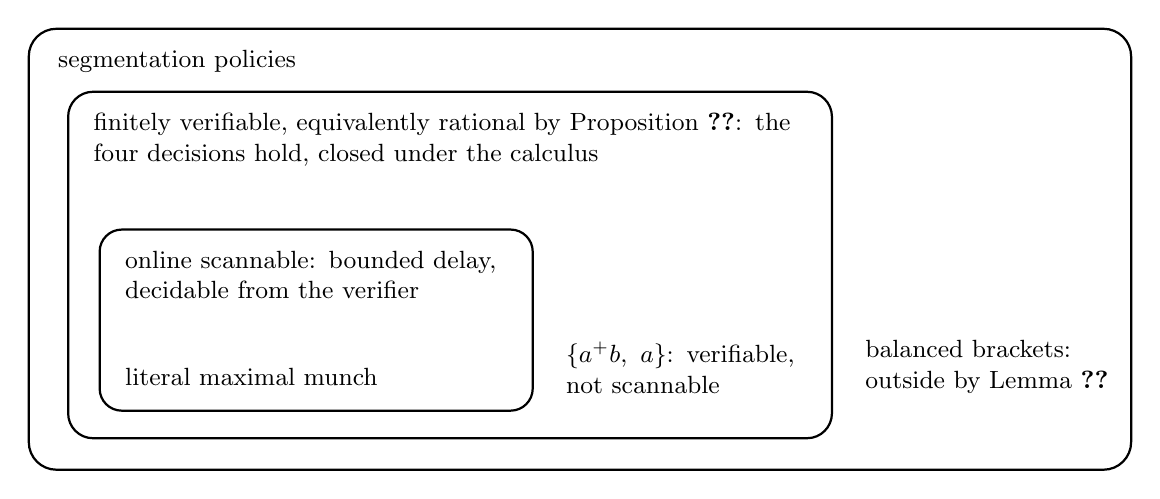
\begin{tikzpicture}[every node/.style={font=\small}]
\draw[rounded corners=10pt, thick] (0,0) rectangle (14.0,5.6);
\node[anchor=north west] at (0.25,5.45) {segmentation policies};
\draw[rounded corners=9pt, thick] (0.5,0.4) rectangle (10.2,4.8);
\node[anchor=north west, text width=9.3cm] at (0.7,4.65)
    {finitely verifiable, equivalently rational by Proposition~\ref{prop:collapse}: the four decisions hold, closed
    under the calculus};
\draw[rounded corners=8pt, thick] (0.9,0.75) rectangle (6.4,3.05);
\node[anchor=north west, text width=5.2cm] at (1.1,2.9)
    {online scannable: bounded delay, decidable from the verifier};
\node[anchor=south west, text width=3.4cm] at (6.7,0.85)
    {$\{a^{+}b,\ a\}$: verifiable, not scannable};
\node[anchor=south west, text width=3.2cm] at (10.5,0.85)
    {balanced brackets: outside by Lemma~\ref{lem:outside}};
\node[anchor=south west] at (1.1,0.95) {literal maximal munch};
\end{tikzpicture}
\caption{The landscape the hypothesis draws. Verification is strictly weaker than scanning, and the frontier between
them is decidable. Every policy with a non-regular domain, the exhibited context-free segmentation among them, is
provably outside. The theorems hold on the whole middle region, which is exactly the rational segmentation policies.}
\label{fig:landscape}
\end{figure}

\section{The calculus}\label{sec:calculus}

% machine-check: composition_calculus.py (pipeline closure: 1,020 strings across 4 inner-outer
% pairs, the composite verifier equal to the two-stage reference scan on every marking; the
% collapse pair proved equivalent to its flattened atom and inequivalent with one pair removed,
% differential 'bb' synthesized; restriction closure with ('b', 0) refuted globally over {ab, b}
% and certified on the b-only schema; composite decisions running unchanged on a pipeline;
% splitter closure: 3,094 strings across 3 inner sets, the one-byte-buffer composite verifier
% equal to the per-run reference scan; fallback union proved equal to its union atom).

Real systems rarely run one policy. A pre-tokenizer splits at class changes, a subword stage re-segments each run, a
schema restricts the inputs a stage can see, and a byte fallback totalizes a partial vocabulary. The class is closed
under all of it.

\begin{definition}[Labeler]\label{def:labeler} A \emph{labeler} for a policy is a deterministic finite automaton over
bytes, run from its initial state on each segment's bytes, that names the segment when it closes by a map from its
states to a finite name alphabet. A literal vocabulary supplies a labeler directly, by spelling, and a regular one by
least accepting index. A finite token alphabet alone does not, so the labeler is data that a stage's presentation must
supply.
\end{definition}

\begin{theorem}[Closure]\label{thm:calculus} Finitely verifiable policies are closed under four operations. A
\emph{pipeline} over a stage one presented with a labeler feeds each closed stage-one token to a second policy as its
name. A \emph{restriction} limits the inputs to a regular schema. A \emph{splitter pre-tokenizer} forces boundaries at
character-class changes and runs the inner policy on each run in isolation. A \emph{fallback union} totalizes a literal
vocabulary with single-byte tokens. Each composite verifier is constructed explicitly, and every composite inherits the
four decisions of Theorem~\ref{thm:four} unchanged, together with the cut and chunk independence decisions of
Theorems~\ref{thm:cut} and~\ref{thm:chunk} for the pairs it certifies and the inventories of them.
\end{theorem}

\begin{proof}[Proof sketch]
Pipelines are the construction with content. Pipeline composition requires a supplied finite-state labeler with a finite
name alphabet, and stage two reads that alphabet. A literal vocabulary can use its token spellings as names, so a
spelling labeler's alphabet is stage one's finite token alphabet. A regular vocabulary may have infinitely many
spellings, the closed lexemes $a^n b$ of a regular stage among them, which no finite composite state could carry, so its
presentation must supply an effective finite-state labeler with finite range. The construction takes the labeler as a
parameter, so the closure holds for every labeler a stage is presented with.

Under the hypothesis a composite marked string carries only the composite boundaries, so the composite verifier must
judge stage one's segmentation without seeing its marks. It runs the subset construction on guessed marks, tracking the
finite set of triples of stage-one verifier state, labeler state, and stage-two verifier state consistent with the bytes
read and the composite marks seen, beside one bit recording whether any byte has been read at all. Whenever a tracked
guess closes a stage-one segment, the labeler's name for it is fed to stage two and the labeler resets. At end of input
a tracked triple that has read something feeds its final segment's label to stage two with the non-closing bit before
asking both stages' acceptance; one that has read nothing asks both stages about the empty input and feeds no label. The
consumed-input bit is the construction's own memory, never an inspection of the inner policy's start representation,
which no interface-faithful account may perform. The tracked set is an element of the power set of a finite cube, so the
composite verifier is finite, and finiteness is the closure proof. Each composite verifier accepts exactly the composite
policy's markings, so it is functional and well formed, and Theorems~\ref{thm:four} to~\ref{thm:chunk}, which take any
such verifier, apply to it unchanged. Acceptance requires a tracked triple in which both stages accept.

The other three constructions are short. Restrictions are the product with the schema's automaton, marks invisible to
the schema side. Splitters force a boundary at every character-class change and run the inner policy on each run in
isolation, and their composite verifier carries a one-byte lookahead buffer, enough to see the class change that forces
a boundary before committing the bit. At a forced boundary the composite bit is one, and the buffered byte reaches the
inner policy with bit zero, since its run ends there, so the inner policy must accept before it restarts on the next
run. Fallback unions are set union of a literal vocabulary with the byte alphabet, a plain policy again, total by
construction.
\end{proof}

Each construction is validated against a composite reference scan on every marking of every small string. The regular
pipeline, its labeler naming each closed segment by its least accepting language index, the same priority the reference
scan uses, is exact on 5{,}080 strings, the literal pipelines on 1{,}020 strings across four pipeline pairs, and the
splitters on 3{,}094 across three splitter configurations. Given the labeler that spells a segment back, the composite
is decided boundary-equivalent to the literal pipeline on every staged pair, and each of the two matches the same
two-stage reference scan over $508$ strings. Given a labeler that names a segment by its length class alone, forgetting
which bytes it read, stage two receives an alphabet coarser than the inner token set, which the literal form cannot be
handed. That difference is one of alphabets only. The composite built over the length-class labeler is decided equal to
the two-gram atom over the alphabet, the single-stage policy the composite flattens to, and the literal form reaches
that same atom by another route, so a coarser labeler shrinks the stage-two alphabet without leaving the literal form's
reach.

% machine-check: none. composition_calculus.py carries the labeler as a parameter and is given two,
% the spelling one and the length-class one, but neither is this example, so the separation below is
% an argument and not an executed one.
Definition~\ref{def:labeler} says the labeler is part of stage one's presentation and not a consequence of it. The
following proposition makes that precise, and the theorem's proof does not use it.

\begin{proposition}[A boundary verifier does not determine the names]\label{prop:labeler}
A finite verifier for a policy's boundaries, together with the fact that its token names are finitely many, does not
determine which name a closed segment carries. Two ordered families can present one policy, so that a single verifier
accepts the markings of both, and still induce labelers that disagree on every segment. A second stage then tells the
two pipelines apart.
\end{proposition}

\begin{proof}
Take the ordered family, a finite list of token languages read in priority order, whose first token language is
$\{\code{a}\}$ under the name $X$ and whose second is $\{\code{a}\}$ under the name $Y$, over the alphabet
$\{\code{a}\}$. Nothing in the definition of an ordered family forbids repeating a language under two names, and read as
a literal vocabulary it would carry one name twice, so it is necessarily a named regular family. Maximal munch with list
priority closes a segment at every byte and names it $X$. Reversing the order closes a segment at every byte and names
it $Y$. The two presentations have the same domain and the same boundary function, so they are one policy in the sense
of Definition~\ref{def:fv} and one verifier accepts the markings of both, while the names differ at every segment. A
stage two that accepts $X^{+}$ and refuses any $Y$ then has domain $\code{a}^{+}$ under the first labeler and the empty
domain under the second, so the composite differs. Names are not scarce here, since there are two of them, and the
obstruction is that the boundary graph records where segments close and not which language closed them, so priority
among equally matching languages is the information it drops.
\end{proof}

The calculus has two immediate uses. First, a two-stage pipeline is proved to agree with the single-stage atom it
flattens to, by the generic boundary decider of Theorem~\ref{thm:four} on the common domain, which for these total
policies is equivalence. With one pair removed the pipeline is proved to differ from that atom, the differential
\code{bb} synthesized by the decider. Second, certification becomes \emph{schema-relative}. The window $(\code{b}, 0)$
is refuted globally over $\{\code{ab}, \code{b}\}$ and certified on the \code{b}-only schema, by the same decider on
both sides of the restriction, so a certificate's meaning under a data contract is computed by the same decider.

\section{Stage-local certificates}\label{sec:transfer}

% machine-check: compositional_certification.py (restriction monotonicity on 12 cases, 7 strict;
% splitter forcing on 504 cases; pipeline boundary subset on 363 composite-tokenizable strings;
% the exact lift equal to the composite decider on 190 regular cases, its 70 refutations re-verified
% against the two-stage reference scan, the per-label condition wrong as a decision on 41 of the 190,
% and the constant-labeler example executed; stack transitivity on 60 three-stage cases).

Certificates computed for one stage survive composition under four laws. Each is proved below, and each is cross-checked
by execution on finite cases against the deciders or, for the boundary-subset law, against an independent reference
scan, the checks named where their counts are quoted. Covering an occurrence correctly, and certifying a window, are the
terms of Definition~\ref{def:cover}, under which the position $p+o$ the origin names is a token start and no token start
follows it inside the occurrence.

\begin{proposition}[Monotonicity]\label{prop:monotone}
If $P$ certifies $(W,o)$, so does its restriction to any regular schema $K$.
\end{proposition}

\begin{proof}
The restriction's domain is $\mathrm{dom}(P) \cap K$ and its segmentation of each string is $P$'s, so every occurrence
it must cover is one $P$ already covers correctly.
\end{proof}

Restriction only adds certificates. The global certified set is a subset of the restricted one on all 12 staged cases, 7
strictly, so a global certificate is reusable under every schema.

\begin{proposition}[Splitter forcing]\label{prop:splitter}
Let $S$ be the splitter over a class function $\kappa$ and any inner policy, and let $W$ have length $h \ge 2$ with
$\kappa(W_{h-2}) \neq \kappa(W_{h-1})$. Then $S$ certifies $(W,\,h-1)$.
\end{proposition}

\begin{proof}
The splitter cuts its input into maximal same-class runs and segments each run in isolation, so every token lies inside
one run and every position at which the class changes is a token start. At an occurrence of $W$ at $p$ the bytes at
$p+h-2$ and $p+h-1$ differ in class, so $p+h-1$ is a token start, and since it is the occurrence's final position no
token start lies beyond it inside the occurrence.
\end{proof}

A window whose final byte follows a class change is thus certified at that final position whatever the inner policy
runs, on all 504 staged final-position cases. That is the splitting companion's anchor supply turned into a closure
operation. The stronger any-offset statement is false, and the paper's own decider refutes it, while the final-position
statement holds.

\begin{proposition}[Boundary subset]\label{prop:subset}
For a pipeline $P = P_2 \circ_\lambda P_1$ over a labeler $\lambda$, $\mathrm{dom}(P) \subseteq \mathrm{dom}(P_1)$, and
for every $x \in \mathrm{dom}(P)$ the token starts of $P(x)$ are a subset of those of $P_1(x)$.
\end{proposition}

\begin{proof}
By the construction of Theorem~\ref{thm:calculus}, $P$ is defined where $P_1$ is and $P_2$ accepts the label stream
$\lambda^{*}(P_1(x))$, and the pipeline segments $x$ by grouping consecutive stage-one segments as $P_2$ groups their
labels, so every composite token starts where some stage-one segment starts.
\end{proof}

A pipeline only removes boundaries, on all 363 composite-tokenizable strings of the staged pairs, so a composite
certificate never lands off an inner boundary. The fourth law is a decision rather than an inequality. Write $\Gamma$
for the labeler's finite name alphabet. A \emph{flagged stream} is a word over $\Gamma \times \{0,1\}$ with exactly one
flag set. When a flagged stream is the label stream of $P_1(x)$ flagged on segment $k$, it records that $x$'s $k$-th
stage-one segment is the one in question.

\begin{theorem}[The lift]\label{thm:lift}
Let $P = P_2 \circ_\lambda P_1$ and fix a window $(W,o)$. Let $R \subseteq (\Gamma \times \{0,1\})^{*}$ be the set of
flagged streams obtained by taking $x \in \mathrm{dom}(P_1)$ and an occurrence at $p$ of $W$ in $x$ that $P_1$ covers
correctly, and flagging $\lambda^{*}(P_1(x))$ on the segment that begins at $p+o$. Let
$L \subseteq (\Gamma \times \{0,1\})^{*}$ be the set of flagged streams in $\mathrm{dom}(P_2)$ whose flagged index is
not a token start of $P_2$'s segmentation. Both are regular, $R$ effectively from $P_1$'s verifier, the labeler and the
window, and $L$ from $P_2$'s verifier alone. A stream in $R \cap L$ is the flagged stream of some string on which $P$
refutes $(W,o)$. If $P_1$ covers every occurrence of $W$ in every string of $\mathrm{dom}(P)$ correctly, in particular
if $P_1$ certifies $(W,o)$, then $P$ certifies $(W,o)$ if and only if $R \cap L = \emptyset$.
\end{theorem}

\begin{proof} \emph{$R$ is regular.} Run $P_1$'s verifier on bytes with guessed marks, the labeler beside it, reset at
every closed segment, and beside both the matcher of the certification proof, which tracks the window's match progress
and the token-start indicators of the last $h$ positions. Designate one occurrence nondeterministically at its final
byte, provided the indicators show a start at the origin's position and none after. The segment open at that byte is
then the one beginning at $p+o$, and it is flagged when it closes, at that byte's own mark, a later one, or end of
input. Emit each closed segment's label with its flag. The device is finite, so its accepted runs form a regular
language, and $R$ is the image of that language under the erasing morphism that keeps the emissions, regular again.
\emph{$L$ is regular.} Run $P_2$'s verifier on the stream with guessed marks, carrying whether the next index is a token
start, true at index zero and thereafter the previous mark. On the flagged symbol, latch whether that bit was false.
Accept when $P_2$ accepts with the latch set, and project the marks away.

\emph{Refutation.} Let $(\gamma, k) \in R \cap L$, and take $x \in \mathrm{dom}(P_1)$ and an occurrence at $p$ whose cut
$p+o$ begins segment $k$ with $(\gamma, k)$ as the stream flagged there, which exist since $(\gamma, k) \in R$. The
labeler need not be injective, so $x$ is one such string and not necessarily the only one. Since
$\gamma \in \mathrm{dom}(P_2)$, $x \in \mathrm{dom}(P)$; since $k$ is no token start of $P_2(\gamma)$, $p+o$ is no token
start of $P(x)$, and $P$ covers that occurrence wrongly.

\emph{Certification.} Suppose $R \cap L = \emptyset$, and take $x \in \mathrm{dom}(P)$ with an occurrence at $p$. By
hypothesis $P_1$ covers it correctly, so $p+o$ begins some segment $k$ and the stream flagged there lies in $R$. That
stream lies in $\mathrm{dom}(P_2)$ and not in $L$, so $k$ is a token start of $P_2$'s segmentation and $p+o$ one of
$P(x)$. No token start of $P(x)$ lies in $(p+o,\,p+h-1]$, every one being a start of $P_1(x)$ by
Proposition~\ref{prop:subset} and none of those lying there. Hence $P$ covers the occurrence correctly.
\end{proof}

Emptiness of $R \cap L$ is reachability in the product of the two automata. The product runs over the $R$-device's own
byte moves, the $L$ side stepping only at the labels those moves emit, so a reaching path projects to a refuting byte
string and not only to its label stream, and that projection is the counterexample. $R$ depends only on the labeled
inner stage and $(W,o)$, and $L$ only on the outer policy, so the two automata are stage-local. Thus $R$ can be built
once per window and origin and reused across outer policies. The instrument builds both languages for regular inner
stages, under the labeler that names a segment by its least accepting language index, the priority the reference scan
uses, and for literal outer stages. It holds the product's verdict to the composite decider, that is, the composite
verifier of Theorem~\ref{thm:calculus} under the generic certification decision, on all 190 (inner stage, outer policy,
certified window) cases, and its 70 refutations read back to byte strings the two-stage reference scan tokenizes and
covers wrongly. Its reach is shown by execution. Over inner \code{a} and \code{b} with outer tokens \code{0}, \code{1}
and \code{0000000\,1}, the window $(\code{ab}, 1)$ is refuted by the eight-byte counterexample \code{aaaaaaab}, the
composite decider's own, which no enumeration of streams to length seven contains.

\Needspace{6\baselineskip}
\begin{corollary}[The per-label condition]\label{cor:labels}
In the setting of Theorem~\ref{thm:lift}, with $P_1$ covering every occurrence of $W$ in $\mathrm{dom}(P)$ correctly and
$P_2$ literal over $\Gamma$, call a label \emph{realized left of the boundary} when some stream of $R$ carries it
immediately before its flagged segment. If no such label occurs as a non-final symbol of a token of $P_2$, then $P$
certifies $(W,o)$. When $P_1$ is literal, every label realized left of the boundary is the image under $\lambda$ of a
\emph{compatible left token}, an inner token $t$ whose suffix of length $\min(|t|, o)$ equals the suffix of $W[0..o)$ of
that length, so testing those images instead is a stronger sufficient test.
\end{corollary}

\begin{proof}
Suppose $(\gamma, k) \in R \cap L$. Index zero is always a token start, so $k \ge 1$ and $\gamma_{k-1}$ is realized left
of the boundary. Since $k$ is no token start of $P_2(\gamma)$, the token of $P_2$ covering index $k-1$ covers $k$ as
well, so $\gamma_{k-1}$ is a non-final symbol of it, against the hypothesis. Hence $R \cap L = \emptyset$ and
Theorem~\ref{thm:lift} applies. For literal $P_1$ the segment ending at $p+o$ is a token $t$ occupying
$[p+o-|t|,\,p+o)$, which meets the window's first $o$ bytes on $[\max(p,\,p+o-|t|),\,p+o)$, an interval of length
$\min(|t|, o)$, and agrees with them there, so $t$ is compatible and $\gamma_{k-1} = \lambda(t)$.
\end{proof}

Neither literalness is used beyond a finite vocabulary. The first part needs only that every segment of $P_2$ is a word
of a known finite set $V$ over $\Gamma$, the hypothesis then reading that no label realized left of the boundary occurs
as a non-final symbol of a word of $V$. The second part needs only that every segment of $P_1$ is a word of a known
finite set $U$, every realized label then being $\lambda(t)$ for a compatible $t \in U$. The proof above uses nothing
more, and in that form the corollary covers towers, whose stages have finite vocabularies.

The condition is about labels and not spellings, and the point is executed. Take inner $\{\code{a}, \code{b}\}$ with
every segment given one label, call it $Z$, and outer tokens $ZZ$ and $Z$. The inner window $(\code{ab}, 1)$ is
certified, and no compatible left token's spelling is carried non-finally, so the spelling test grants the lift. The
exact decision refutes it with \code{ab} as the counterexample, since the outer stream is $ZZ$ and maximal munch takes
it whole. The compatible tokens reach outside the window for a reason of the same kind. Over inner
$\{\code{aa}, \code{a}, \code{b}\}$ the occurrence in $\code{aab}$ ends the token $\code{aa}$ at a boundary whose window
shows only $\code{a}$. Nor is the condition necessary. Over inner $\{\code{a}, \code{b}\}$ with outer tokens
$(\code{a},\code{a})$, $(\code{a})$, $(\code{b})$, the window $(\code{ab}, 1)$ lifts although \code{a} is carried
non-finally, because the window fixes the following symbol and the merge the condition fears is unreachable in its
context. In general the condition falls short because it reads what can stand left of the boundary and not what the
window and the inner stage allow to follow it, so a token carrying the left label non-finally can be unrealizable at the
boundary. Evaluated over the labels the product realizes, the condition grants no lift the composite refuses and is
wrong as a decision on 41 of the 190 staged cases.

The lift also answers a dictionary update. Take the byte-pair table with the one merge $\code{b}+\code{c}$ over the
alphabet $\{\code{a}, \code{b}, \code{c}\}$ and extend it by the merge $\code{a}+\code{b}$ at the later rank, so that
the extended table tokenizes \code{abc} as \code{a} then \code{bc}, the earlier rank winning. The window $(\code{b}, 0)$
is certified under the one-merge table and refuted under the extended one by the counterexample \code{ab}, one token,
whose \code{b} is covered by a token beginning before it, while the window $(\code{abc}, 1)$ is certified under both.
The update is a pipeline in which the one-merge tower, whose single stage is the literal set
$\{\code{a}, \code{b}, \code{c}, \code{bc}\}$, sits below a literal stage over those token names that carries the new
merge as the token $(\code{a}, \code{b})$, each segment named by its spelling. Its reference segmentation equals the
extended table's on all 3{,}280 strings through length 7.

On the surviving certificate the per-label condition refuses the lift, since the label \code{a} is realized left of the
boundary and carried non-finally by $(\code{a}, \code{b})$, while the exact lift proves it, the product of the two
stage-local automata being empty and the composite decider agreeing. At an occurrence of \code{abc} the inner stage
supplies \code{a} followed by \code{bc}, so the outer token $(\code{a}, \code{b})$ cannot cross the marked boundary. The
product built for $(\code{b}, 0)$ refutes that window by the counterexample \code{ab}.

The two greedy disciplines separate on the same window. Literal maximal munch over the extended table's final vocabulary
$\{\code{a}, \code{b}, \code{c}, \code{ab}, \code{bc}\}$ tokenizes \code{abc} as \code{ab} then \code{c}, so the generic
decision certifies $(\code{abc}, 1)$ on the tower and refutes it on the literal policy with \code{abc} as the
counterexample. A certificate is a statement about one policy, and a table and the longest match over its vocabulary are
two.

\begin{proposition}[Stack transitivity]\label{prop:stack}
Let $C = T \circ G$ be a tower of pipelines, $T$ reading $G$'s segments through a labeler as in Theorem~\ref{thm:lift},
whose innermost stage certifies $(W,o)$. Then $C$ certifies $(W,o)$ if and only if $G$ covers every occurrence of $W$ in
every string of $\mathrm{dom}(C)$ correctly and $R_G \cap L_T = \emptyset$, with $R_G$ and $L_T$ the languages of
Theorem~\ref{thm:lift} for $G$ and $T$.
\end{proposition}

\begin{proof}
By Proposition~\ref{prop:subset} at each level, the token starts of $C(x)$ lie among those of $G(x)$, which lie among
the innermost stage's, and the innermost certificate leaves no start in $(p+o,\,p+h-1]$ for any occurrence at $p$ in any
$x \in \mathrm{dom}(C)$, so $G$ covers such an occurrence correctly exactly when $p+o$ starts a token of $G(x)$, and $C$
exactly when $p+o$ starts one of $C(x)$. If $G$ covers every occurrence in $\mathrm{dom}(C)$ correctly,
Theorem~\ref{thm:lift} with $P_1 = G$ and $P_2 = T$ gives the equivalence. Otherwise some $p+o$ starts no token of
$G(x)$, hence none of $C(x)$, so $C$ refutes the window and both sides fail.
\end{proof}

Each level of a tower is thus asked its own question, the quantifier running over the tower's own domain, and both
premises are necessary. A top stage that rejects the stream carrying a violation of $G$ hides it from $C$, so the
quantification must run over $\mathrm{dom}(C)$ and not $\mathrm{dom}(G)$. A top stage that merges the window's bytes
into one token repairs a violation of $G$, so without the innermost certificate the equivalence fails. Both are staged,
and the equivalence is checked by enumeration on 60 three-stage cases.

\section{The weighted theory}\label{sec:weighted}

% machine-check: weighted_general.py (the general route: the trimmed product of the raw verifier
% with the source built through the interface, the spectral bound certified by an exact nonnegative
% inverse of I - A, the multiplicity lemma and the path-mass bound checked by enumeration, on 25
% literal sets under two sources, 29 of the 50 cases carrying a row above one, 15 memoryless and 14
% two-state, equal to the deterministic engine on every literal set, and on the regular example
% without an online scanner and a two-mode instance within brute-force tails; the deterministic
% engine against enumeration over the literal family; the raw rho-equals-one verifier singular
% untrimmed and recovered trimmed; the boundary cases returning exact zeros and refusing a source
% with an endless branch; the pair route over (source, verifier, verifier, disagreement) with
% paired marks and mismatch rewards, equal to weighted_shadow's differential automaton on 100
% ordered literal pairs and bracketing brute force on the mixed and regular pairs beyond it);
% weighted_shadow.py (30 exactness triples, dynamic program equal to enumeration to
% the digit, residuals exactly zero, enclosures bracketing; the positivity law on 100 ordered
% pairs; the one-merge extension's closed forms 4/11 and 1/5); markov_shadow.py (the one-state
% lift equal rational for rational; 12 Markov exactness triples; the refined positivity law on 60
% (pair, source) cases with 2 support-erasure cases; the corpus-digram closed form
% 3396201545233/54186662216209 against 833/2561 matched uniform).

The decisions say whether; deployment asks how often. The hypothesis of this section covers every well-formed functional
verifier presenting a policy, in the sense of Theorem~\ref{thm:four}, under a rational, unifilar, almost surely stopping
finite-state source, unifilar meaning that the current state and the byte emitted determine the next state. A memoryless
byte source with rational byte probabilities and a positive rational stopping probability is the one-state case, and
Proposition~\ref{prop:weighted-general} shows that the theorem holds without unifilarity. Token counts below follow the
final-zero convention of Section~\ref{sec:interface}. For a nonempty string, the token count is the number of set
boundary bits plus one; the empty string has zero tokens. Differential mass between two policies is the mass of the
strings of their common domain that they segment apart, and the per-byte rates are ratios of expectations, differing
positions in expectation over expected length, which keeps them rational where an expectation of per-string ratios would
not be.

\begin{theorem}[Exact weighted shadow]\label{thm:weighted} Let $V$ be a well-formed functional finite verifier
presenting a policy, and let $S$ be a finite-state byte source with rational transition and stopping probabilities,
unifilar, and almost surely stopping. The following are rational: the tokenizability mass of $V$ under $S$; the
unnormalized expected length and expected token and boundary counts contributed by accepted strings; and, for a second
such verifier $V'$, the differential mass and the unnormalized expected length and number of mismatched boundary bits on
the common domain. Each is zero when the product has no live state. Otherwise each is the start-state coordinate of the
unique solution of an affine system $x = Ax + b$ over the live states of the product of $V$, or of $V$ and $V'$, with
$S$, where the spectral radius of $A$ is strictly below one. Every rate that is a quotient of two of these expectations
is rational wherever its denominator, an expected length, is positive.
\end{theorem}

\begin{proof}
Each mass and each unnormalized expectation is a vector indexed by the live states of the product of the verifier with
the source, the states reachable from the start from which joint acceptance is reachable, where the verifier accepts and
the source can stop. For the pair quantities the product runs both verifiers over one byte stream with their marks
guessed in pairs and their first disagreement latched. Each such vector satisfies an affine fixpoint $x = Ax + b$ with
coefficients drawn from the byte probabilities and stopping mass, and each rate is the ratio of two start-state
coordinates of such solutions. When no state is live the system is empty, and the mass, the expected length and the
expected counts are zero. Those systems are absorbing chains only in the deterministic presentation, since a raw row can
exceed one.

The bound on the spectrum is where functionality earns its place. On a raw marked verifier both marks of one byte can
remain useful, $\{\code{a}, \code{ab}\}$ after reading $\code{a}$ already does it, and rows of $A$ can exceed one, so
the bound on $A^{n}$ has to come from multiplicity, since row sums give none. Two markings of one byte prefix that reach
the same live state extend, by liveness, along one completion to two accepted markings of one string, which
functionality forbids. Hence the alive markings of a prefix occupy distinct states, at most $N$ of them for $N$ live
states, and the mass of the paths of length $n$ is at most $N$ times the probability that the source emits at least $n$
bytes. For the quantities solved over the product of two verifiers a marking is a pair of markings, and the same
argument runs on whichever component the two differ in. From every state it enters with positive probability, a
finite-state source that stops almost surely has a positive probability of stopping within $m$ steps, $m$ its state
count. Those states are finitely many, so the least of these probabilities is a $\delta > 0$, and the probability of
emitting at least $n$ bytes decays geometrically over blocks of $m$ steps, by a factor of $1 - \delta$ per block, so its
sum over $n$ is finite. The Neumann series $\sum_n A^{n}$ therefore converges from the start state, hence from every
live state, each reachable from the start with positive mass, and the spectral radius sits strictly below one, so the
solution is unique. Where a deterministic online presentation exists and every source state stops with positive
probability, one successor per byte keeps every row at most one minus the stopping probability and the same bound
follows in a line. Rational coefficients keep the unique solution rational, and a quotient of two rationals with
positive denominator is rational. \end{proof}

\begin{proposition}[Positivity]\label{prop:positivity} Under the hypotheses of Theorem~\ref{thm:weighted}, the
differential mass of $V$ and $V'$ under $S$ is positive exactly when the boundary half of the equivalence decision of
Theorem~\ref{thm:four}, run on the restrictions of $V$ and $V'$ to the support of $S$, returns a differing string.
\end{proposition}

\begin{proof}
The support of $S$, the strings it emits with positive probability, is a regular language, recognized by the source's
states with its positive-probability transitions, accepting where the stopping probability is positive. Differential
mass is a sum of nonnegative terms, one per string of the common domain that the two policies segment apart, each that
string's probability under $S$, so it is positive exactly when some such string lies in the support. A differing string
through a zero-probability byte carries no mass. The restrictions of $V$ and $V'$ to the support are verifiers by
Theorem~\ref{thm:calculus}, with the common domain cut down to the support and the segmentations unchanged, so the
boundary half run on them returns a differing string exactly when such a string exists.
\end{proof}

The measure and the logic thus agree about zero, on the boundary half alone, since the measured event is disagreement on
the common domain. Two policies whose domains differ while their shared segmentations agree carry zero differential mass
and are still separated by the domain half, which the law does not speak about. Under a full-support source, one in
which every byte and the stop carry positive probability, the restriction is the identity and the law reads plainly.

The theorem itself holds for sources in which one state and one byte lead to several next states, provided each
transition emits exactly one byte.

\begin{proposition}[Sources need not be unifilar]\label{prop:weighted-general} Theorem~\ref{thm:weighted} and
Proposition~\ref{prop:positivity} hold for every finite-state byte source $S$ with rational probabilities on its
byte-labeled transitions and on stopping that emits exactly one byte per transition and stops almost surely, whether or
not $S$ is unifilar.
\end{proposition}

\begin{proof}
Of the proofs of Theorem~\ref{thm:weighted} and Proposition~\ref{prop:positivity}, the product's definition and the
bound on the spectrum use unifilarity, where a byte prefix determines the source's run, so both are rebuilt here. Build
the product over pairs of a source state and a verifier state, with one edge for every source transition of positive
probability and every mark the verifier admits on its byte, weighted by the transition's probability, and trim it to its
live states. A string's probability is the sum of the weights of the source runs that emit it and stop, and
functionality gives its bytes at most one accepted marking, so the masses and expectations are again start-state
coordinates of affine systems $x = Ax + b$ over the live states. Fix a run of $S$ through $n$ transitions. Two distinct
marking paths along it that reach one verifier state at a live product state extend, along one source continuation and
one marked completion to joint acceptance, to two accepted markings of one string, which functionality forbids. The live
marking paths along the run therefore occupy distinct verifier states, at most $|Q|$ of them for the verifier's state
set $Q$, and summed over the runs the mass of the product's paths of length $n$ is at most $|Q|$ times the probability
that $S$ emits at least $n$ bytes. For the pair quantities a path carries a pair of markings, and two distinct pairs
reaching one pair of verifier states at a live product state differ in a component that would receive two accepted
markings of one string, so at most $|Q|\,|Q'|$ pairs live along each run, $Q'$ the second verifier's state set. The
block bound in the proof of Theorem~\ref{thm:weighted} uses only that $S$ is a finite Markov chain on its states that
stops almost surely, so the probability of emitting at least $n$ bytes decays geometrically over blocks, the Neumann
series converges from the start state and from every live state, the spectral radius of $A$ is below one, and each
solution is unique and rational. For positivity, the source's positive-probability transitions, accepting where the
stopping probability is positive, now form a nondeterministic automaton, whose language, the support of $S$, is still
regular, so the proof of Proposition~\ref{prop:positivity} runs unchanged on the restrictions to it.
\end{proof}

The executable interface of this paper remains unifilar. Its source objects present one successor per state and byte,
and the solver and its checks below run on those, so Proposition~\ref{prop:weighted-general} is proved here and not
claimed as implemented.


The solver solves each system exactly over the rationals and asserts the residual $x - (Ax + b)$ zero coordinate by
coordinate, and the dynamic program is held equal, to the digit, to per-string enumeration on 30 staged triples. The
deterministic engine serves the literal instances, while the regular-token example of Section~\ref{sec:real}, which has
no online scanner, and the two-mode instance are decided by the trimmed product alone, cut down to its live states.
Raw-product validation is split by family, with the memoryless literal cases and the literal pairs compared with their
exact deterministic engines, the two-state literal cases checked by exact inverse and residual identities and by finite
multiplicity and path-mass tests, and the regular and two-mode single-policy cases and the pair cases beyond the literal
path bracketed by finite enumeration with exact tails. Unifilar Markov sources carry every quantity over by the same
methods. The block-survival bound above replaces the memoryless one-step tail, the solver refuses a source that does not
terminate and gives its reason, and on a one-state source it returns exactly the rationals of the memoryless solver it
generalizes. The positivity law is checked in its plain form on 100 ordered pairs under a full-support source, and in
its support-refined form, with the right-hand side computed by the paper's own restriction calculus, on 60 pairs of
policy pair and source, including two erasures where a globally differential pair has mass exactly zero because the
support forbids every differing string.

Two closed forms show the instrument's reach. Both are outputs of the same solved systems, reported without separate
enclosures of their own. The one-merge extension $\{\code{a}, \code{b}, \code{ab}\}$ to
$\{\code{a}, \code{b}, \code{ab}, \code{ba}\}$ under a memoryless source has differential probability exactly $4/11$ and
per-byte mismatch rate $1/5$ under $P(a) = P(b) = 2/5$ and $P(\mathrm{stop}) = 1/5$, where the earlier experiments
sampled. The analogous extension $\{s, q, o, qo\}$ to $\{s, q, o, qo, os\}$ over the three classes structural, quote and
other, under corpus digram statistics, has differential mass about $0.063$, exactly $3396201545233/54186662216209$,
against $833/2561$, about $0.325$, under the matched uniform source. The measure moves with the world it models, in
closed form. The comparison is matched by design. The digram conditionals carry no smoothing weight, both sources stop
with probability exactly $1/8$ at every state, the corpus start state is the first byte's class, and the uniform
comparator's expected length, exactly seven, equals the corpus source's, so one comparator is matched on stopping and on
length at once. Corpus structure, on this slice, concentrates mass on strings where the two vocabularies agree.

\section{Instances and applications}\label{sec:instances}

% machine-check: segmentation_equivalence.py (the vocabulary upgrade differential: 320 tokens
% against 352, a boundary-breaking string of length 2, the corpus read byte for byte); the running
% instances of the two companions are measured in their own papers and are not duplicated here.
The empirical weight of this series lives in its two companions and stays there. The recovery companion measures
certified recovery against the classical conventions on archived campaigns, and the splitting companion measures anchor
supply, splits the recovery campaign's archived corpus at certified anchors with a threaded scanner, and decides its own
design change with a synthesized differing string. This paper keeps the instances that belong to the abstraction, and
one measurement its own lift invites. A vocabulary upgrade from 320 to 352 tokens produces a boundary differential, a
differing string of length two. The tokens are byte-pair merges over the full byte alphabet, trained on the JSON sample
the programs read, simdjson's \code{twitter.json}. That file is fetched from its pinned release, held to its digest and
read byte for byte. The added merges silently reframe two bytes, the cached-segmentation hazard exhibited by
construction. Byte-pair encoding is an exact instance of the class. Canonical BPE has the finite-state constructions of
\citet{cognetta2025tokenization} and \citet{berglund2024bpedfa}. For a proper dictionary, one whose every multi-symbol
merge part is an earlier merge's product, the construction of \citet{berglund2024bpedfa} is a subsequential transducer
from strings to tokenizations by Theorem~4 of that paper's extended version. Writing each emitted token $u$ as the mask
$0^{|u|-1}1$ and closing the output with a zero bit in place of the last one keeps that transducer subsequential and
length-preserving, so the bridge of Section~\ref{sec:real} places such a policy inside the online-scannable region, and
the four decisions apply to it directly. Canonical BPE is nonetheless not in general a maximal-munch policy, for the
reason Section~\ref{sec:related} records.

% machine-check: bpe_transfer_study.py, both dictionaries from their stored records (base 64 merges, extensions 1, 2, 4, 8, 16;
% JSON inventory 3740 pairs, 1174 certified, 2566 refutations replayed; GPT-2 inventory 2684 pairs, 902 certified,
% 1782 replayed; (a) = (c) and (b) a subset of (a) at every k; the supply, gap and cost lines of data/bpe-transfer-study.txt
% and data/bpe-transfer-study-gpt2.txt are the table's rows).
The lift of Theorem~\ref{thm:lift} answers a question a growing dictionary asks of every certificate it holds, whether
the certificate survives the next merges. Appending merges is one way pretrained tokenizers are adapted.
\citet{purason2026teaching} continue a tokenizer's BPE training on new data, \citet{smith2026inplace} continue its
merges in place, and \citet{herold2025vocabulary} add domain tokens under a guarantee that no input tokenizes longer,
but none of them asks which certificates survive. The exploration decides it on byte-pair dictionaries of 64 merges
extended by the next $k$ merges of their own training, for $k$ from 1 to 16. It runs two dictionaries side by side, one
trained on the corpus and the other the first merges of the GPT-2 table, applied to raw bytes without GPT-2's
pre-tokenizer. In the GPT-2 table the appended merges with the space byte as left part number 1 among the first 8
appended and 3 among the first 16.

The verifier is a deterministic tower, one single-lookahead transducer per merge composed into one automaton, since the
subset-construction tower behind the byte-pair policies of Section~\ref{sec:four} passes 5{,}000 states within two
merges. The deterministic tower has 4{,}063 states for the corpus dictionary and 561 for the GPT-2 prefix over the bytes
some merge names and one inert stand-in for the rest, a reduction that is sound because a byte no merge names is only
ever a single-byte token and no merge joins across it, and that is checked against the full byte base on 48 sampled
pairs. The tower requires that every merge produce a token distinct from the alphabet and from every earlier product, as
both trained tables do. The verifier is held to the reference encoder on exhaustive sweeps over the five byte-pair
universes of Section~\ref{sec:four} and 12 random tables, 2{,}555 and 22{,}746 strings, to the subset tower on those
universes, and to the reference markings of 171 held-out pieces, which the longest extension's tower accepts while
refusing every one of their 8{,}037 single-mark perturbations.

The inventory is frozen before any extension is decided and holds every window of width one to three, with every origin,
in a 16 KiB slice held out from training, 3{,}740 pairs for the corpus dictionary and 2{,}684 for the GPT-2 prefix, of
which the base towers certify 1{,}174 and 902, the 2{,}566 and 1{,}782 refutations replayed by the encoder. The anchor
supply is measured on the next 16 KiB. Each certificate is then decided three ways under every extension: by the
composite decision on the extended tower; by the exact lift, the inner stage the base tower and the outer stage the
tower of the appended merges over base token names, a pipeline whose marked language equals the extended tower's,
checked at $k = 16$, with $R$ built once per certificate from the base tower and $L$ from the outer tower's verifier;
and by the compatible-token test of Corollary~\ref{cor:labels}, its stronger second part, in the finite-vocabulary form
stated after it, with the base-token spellings of all outer tokens as the outer vocabulary, each base token, the single
bytes among them, spelled as itself and each appended product as the base tokens it concatenates. The test is coarser
than the per-label condition it bounds, which reads the labels realized left of the boundary. Over
$\{\code{a}, \code{b}\}$ with the base merge $\code{a}+\code{a}$ and the appended merges $\code{a}+\code{b}$ and
$\code{a}+\code{aa}$, the window $(\code{baaa}, 3)$ is certified by both towers and by the exact lift, its only realized
label is \code{aa} and the per-label condition grants it, while the compatible tokens include \code{a}, which the new
token $(\code{a}, \code{b})$ carries non-finally, and the test refuses it. Table~\ref{tab:transfer} has the counts. The
exact lift equals the composite decision on every certificate of every extension, and the test grants nothing the lift
refuses. Of what the test discards, the lift keeps 474 certificates of the corpus dictionary at $k = 16$ and 236 of the
GPT-2 prefix.

\begin{table}[tp]
\centering
\small
\begin{tabular}{llrrrrrrr}
\toprule
Dictionary & $k$ & \multicolumn{2}{c}{Kept} & Recovered & \multicolumn{2}{c}{Anchors per KiB} & Anchor gap &
Longest \\
\cmidrule(lr){3-4} \cmidrule(lr){6-7}
  & & exact & test & & exact & test & p99 & stretch \\
\midrule
JSON & base & 1{,}174 & & & 482.4 & & & \\
 & 1 & 1{,}168 & 1{,}132 & 36 & 480.1 & 476.4 & 17 / 17 & 22 / 22 \\
 & 2 & 1{,}162 & 1{,}068 & 94 & 478.0 & 462.8 & 17 / 17 & 22 / 24 \\
 & 4 & 1{,}152 & 969 & 183 & 472.2 & 428.2 & 17 / 17 & 22 / 24 \\
 & 8 & 1{,}136 & 799 & 337 & 461.9 & 365.9 & 20 / 21 & 30 / 32 \\
 & 16 & 1{,}111 & 637 & 474 & 446.6 & 313.8 & 20 / 23 & 30 / 42 \\
\addlinespace
GPT-2 & base & 902 & & & 927.9 & & & \\
 & 1 & 898 & 846 & 52 & 923.7 & 914.2 & 2 / 3 & 5 / 7 \\
 & 2 & 895 & 811 & 84 & 922.2 & 902.3 & 2 / 3 & 5 / 7 \\
 & 4 & 889 & 784 & 105 & 920.6 & 887.8 & 2 / 3 & 5 / 7 \\
 & 8 & 878 & 710 & 168 & 914.2 & 615.7 & 2 / 11 & 5 / 20 \\
 & 16 & 867 & 631 & 236 & 909.0 & 574.9 & 2 / 11 & 5 / 20 \\
\bottomrule
\end{tabular}
\caption{Base certificates of a dictionary of 64 merges that survive its next $k$ merges, decided three ways, by the
composite decision, the exact lift and the compatible-token test; the first two agree on every certificate and share the
column exact, and test is the compatible-token test. Kept counts the surviving certificates of the frozen inventory and
recovered those the lift keeps that the test discards; anchors per KiB, the 99th-percentile anchor gap, between
consecutive anchors, and the longest anchor-free stretch, both in bytes, are measured on the held-out evaluation slice,
exact against the test where a cell holds two figures, and the base row has no extension to compare. The JSON dictionary
is trained on the corpus; the GPT-2 dictionary is the first merges of the GPT-2 table, whose space-led merges begin at
$k = 8$.}
\label{tab:transfer}
\end{table}

The supply tells where the loss falls. On the corpus dictionary the test's anchors thin steadily, 313.8 per KiB against
the exact lift's 446.6 at $k = 16$, the longest anchor-free stretch 42 bytes against 30, 2{,}126 of 7{,}146 anchor
positions of the evaluation slice recovered by the lift. On the GPT-2 prefix the test's supply falls gently, to 887.8
anchors per KiB at $k = 4$, until the first space-led merge arrives at $k = 8$, and then it falls to 615.7 while the
exact lift goes from 920.6 to 914.2. From there on the test refuses all 11 base certificates whose boundary follows a
space, the space being carried non-finally by the new token, and the lift, which asks instead whether the merge is ever
realized across the boundary, keeps every one of them. At $k = 16$ the exact lift holds 909.0 anchors per KiB against
the test's 574.9, the p99 anchor gap 2 against 11, the longest stretch 5 against 20, and 5{,}346 of 14{,}544 anchor
positions are recovered. Across all five extensions, the exact lift costs less even after including its one-time
construction, 2{,}863.3 against 16{,}112 seconds of summed task time on the corpus dictionary and 652.6 against 1{,}502
on the GPT-2 prefix. For GPT-2 the first extension alone, 425.1 against 249, does not repay the build. The stage-local
automata of the base tower are built once, 1{,}819 and 391 seconds of summed task time outside the factor, and a lift
product over them is cheaper than deciding the extended composite from scratch by a factor of 13.7 to 16.3 on the corpus
dictionary and 4.7 to 7.3 on the GPT-2 prefix, in summed task elapsed time. Over a sample of 24 certificates and the
five extensions, reuse took 108.4s against 658.3s on the corpus dictionary and 26.4s against 66.3s on the GPT-2 prefix.
The compatible-token test is a sound first filter that needs no product search, but after sixteen appended merges it
discards 29.8 and 36.8 percent of the anchor positions the exact lift keeps on the two dictionaries, against at most 9.3
percent through four.

% machine-check: wordpiece_instance.py (the 4,096 prefix: 41 symbols, 29786 verifier states, 4747 pairs, 2065 certified,
% 2682 refuted and replayed, gap 15, no lasso, mask 26211, 466 of 476 occurring certified cuts not independent; the
% full lexical vocabulary: 71 symbols, 138510 states, 1230 certified, 3517 refuted, gap 18, no lasso, 196 of 590
% occurring cuts independent; the records are data/wordpiece-instance.txt and data/wordpiece-instance-full.txt, reported
% from the records unless a rerun is asked for).
WordPiece, the subword tokenization method of \citet{schuster2012japanese}, has a real-vocabulary instance too, at two
depths. The policy is the partial two-mode longest-match lexical policy over the BERT-Base, Uncased vocabulary of
\citet{devlin2019bert}, read on lowercased raw text, its plain entries the initial tokens and its \code{\#\#} entries
the continuation tokens. It is not the end-to-end tokenizer of BERT's reference implementation \citep{bertcode}, because
it omits the basic tokenizer's cleaning, its accent stripping by Unicode decomposition, its splitting on whitespace and
punctuation and its handling of CJK characters, and the \code{[UNK]} fallback with its limit of 200 characters on word
length, and it fails where no token matches. A vocabulary does not determine its inference method, \citet{uzan2024greed}
comparing several over the same vocabularies, so the policy is named by its scan and not by its vocabulary alone.
\citet{song2021fast} compute that scan in linear time from the vocabulary's trie with failure links in the manner of Aho
and Corasick, while here its marked scans are recognized and properties quantified over every string decided on them.
The vocabulary file opens with 999 reserved entries, its special tokens and unused slots, and 997 single characters, and
the first depth takes the next 4{,}096 entries in the file's token-ID order over those 997 characters. Reduced jointly
with the policies it is compared with below, its alphabet is a quotient of 41 symbols, namely 39 named characters, 38 of
them named by its own tokens, and two stand-ins, one for each joint vector of initial and continuation membership that
the remaining characters carry across the compared policies. At this depth \code{<1>} stands for the 957 characters that
every compared policy, the prefix's own among them, holds as single initial tokens and none as continuation tokens, and
\code{<2>} for the one character subscript two, which the deepest comparison also holds as a continuation token.

The reduction is sound. A character that no multi-character token of any compared policy contains can be consumed only
as a single-character token, in the modes its membership vector allows, and no token begun before it reaches across it,
so replacing every such character by another with the same vector leaves every scan's success or failure and every
boundary unchanged. A refuting text over the full base maps to one over the quotient with the same boundaries and the
same occurrence, and a refuting quotient text lifts to a raw one by restoring the raw window's characters at the
distinguished occurrence and writing any representative of its class elsewhere, so a canonical window's verdict is the
verdict of every raw window it stands for. A check of 51 pairs decided both ways, the raw window over all 997 characters
and the canonical one over the quotient, confirms it.

Over the quotient the prefix has a verifier of 29{,}786 states, on which the four decisions take seconds to about a
minute: 4{,}747 window and origin pairs from a held-out slice of \code{twitter.json}, 2{,}065 certified and 2{,}682
refuted with every refutation replayed; a boundary gap of 15, the length of \code{representatives}, with no lasso; a
realizability mask of 26{,}211 states that strands nothing; and the vocabulary one entry deeper separated by the
appended word, \code{electoral}, which the shorter prefix spells \code{el|e|c|tor|al}. The mode is visible in both
differing strings against maximal munch over the same initial tokens, \code{<1>00} segmented apart and \code{<1><1>}
tokenized only without modes, and in the cut decision. Of the 476 occurring certificates, those whose window occurs in
some domain string, 466 are cuts that are not independent, each failing on the suffix side only, a shortest
counterexample \code{<1>ca}.

At full lexical depth, all 28{,}526 entries after the head over the same 997-character base, the 999 reserved entries
excluded, the policy's verifier is built from its two tries, without exploring the scan's configurations, the two
constructions corresponding at the prefix with no transition in disagreement. It has 138{,}510 states over a quotient of
71 symbols, 70 named characters and \code{<1>}, which at this depth stands for the other 927 characters, single tokens
in both modes here and initial ones only at the 4{,}096 prefix. Each quotient symbol is a single-character token in both
modes, so every string over the quotient alphabet is in the policy's domain. On the same 4{,}747 pairs it certifies
1{,}230 and refutes 3{,}517, every refutation replayed. The boundary gap is 18, the length of \code{telecommunications},
with no lasso, the search for one taking 708.1 seconds, and the mask keeps 136{,}766 of 138{,}510 states and strands
nothing. The full-depth policy is separated from the 4{,}096 prefix by \code{02} on the boundaries and \code{<1><1>} on
the domain, and from maximal munch over its own initial tokens by \code{<1>0s} on the boundaries alone, the two domains
coinciding. Of the 590 occurring certificates, 196 are cuts that are independent, every one of them with a stand-in in
its window, and 394 are not, again each on the suffix side only.

Within maximal named-character runs the anchors are few. On the 16{,}384-character evaluation slice, counting only in
the runs the policy tokenizes whole, the prefix policy certifies 597 anchor positions and the full-depth policy 333, or
37.3 and 20.8 per 1{,}024 characters of the full slice, none of them inside a run the scan reads as one token. The runs
start at 1{,}434 positions. Across the 1{,}049 maximal alphabet runs of the raw slice, within which every quotient
symbol is a single-character token in both modes at full depth, the full policy certifies 4{,}853 positions, or 303.3
per 1{,}024 characters of the full slice, the other 5{,}003 characters of which lie outside the alphabet.

% machine-check: library_instance.py (munch at release 2.3.0, commit fa3f20d: the five fixtures the exploration's
% generators write, each held byte for byte to the copy the library's tests read; the decisions' fixture 474 universes,
% 16,116 certifications of which 10,804 refused, 472 finite gaps and 2 lassos, 474 realizability verdicts, 1,818 pairs;
% the cut fixture 489 universes, 16,626 windows at their origins, 11,047 uncertified, 5,517 independent and 62 not;
% the chunk fixture 494 universes, 29,085 inventories, 27,326 chunk-independent and 1,759 not; the merge-tower fixture
% 14 universes and 10,177 strings, the trie-chain fixture 16 universes and 13,713 strings, each with certifications,
% gaps, realizability and pairs; the library's 22 verifier, 8 merge-tower and 6 trie-chain tests passed, the five
% fixture tests among them; the supply probe on twitter.json, 19,434 windows, 53,074 window origin pairs, 284
% certified by the verifier and 267 by the window route, 0 disagreements, 17 conservative refusals all confirmed by
% exact search, 43,043 certified positions, 69.79 per KiB, longest uncertified stretch 464 bytes; the record is
% data/library-verifier.txt, regenerated when a build directory is given and reported from the record otherwise).

The munch lexer library \citep{munch} implements the interface at its release 2.3.0 with a deterministic trim automaton
over marked symbols built from any transition table, the armed run of Section~\ref{sec:interface} over a byte automaton,
and the verifiers the two tokenizer instances above are decided on, the merge tower of canonical byte-pair encoding as
\code{merge\_tower()} and the trie chain of two-mode WordPiece as \code{trie\_chain()}. The library also implements the
four decisions of Section~\ref{sec:four} and the cut and chunk independence decisions of Theorems~\ref{thm:cut}
and~\ref{thm:chunk} as \code{dependence()} and \code{chunk\_dependence()}. Its test suite holds each of them to
reference answers this paper's exploration writes for it. Every counterexample of a refuted window or a failing cut or
chunk, every differing string of a failed equivalence and every lasso, the library's and the fixture's, is replayed
through a reference scan, a reference encoder or the verifier, except the refuting texts the cut fixture records for its
uncertified pairs, which the tests do not read, since an uncertified pair need only be refused. Verdicts that return no
string and boundary-gap suprema are compared, and a realizability mask is checked against co-accessibility state by
state in the fixture of the four decisions but only for its presence and size in the merge-tower and trie-chain
fixtures.

The fixture of the four decisions has 474 universes, every set of one to three distinct words of length one to three
over two symbols and the five regular sets of the edit sweep, and carries 16{,}116 certification decisions, 474
boundary-gap decisions of which 2 are lassos, 474 realizability verdicts and 1{,}818 equivalence pairs. The cut fixture
decides every window of length one to three at every origin over 489 universes, 5{,}517 certified cuts independent and
62 not. The chunk fixture decides 29{,}085 inventories over 494 universes, 1{,}759 of them not chunk-independent. Both
fixtures are the independence sweeps above less their five byte-pair universes, whose tabulated towers run to thousands
of states. The chunk fixture adds one universe of its own, every nonempty string over $\{a, b\}$ segmented byte by byte,
whose start accepts nothing. The merge-tower and trie-chain fixtures hold the two constructions to the reference
encoder's markings of 10{,}177 strings over 14 byte-pair tables and the reference scanner's markings or refusals of
13{,}713 strings over 16 two-mode vocabularies, and pose the four decisions on each.

Given a build of the library at that release, the gate's library stage regenerates the five fixtures and holds each byte
for byte to the library's copy, runs the library's verifier, merge-tower and trie-chain tests and its supply probe, and
writes the record this instance is held to. Without such a build it reports the archived record and names the
regeneration it did not run. On \code{twitter.json} under the JSON grammar the library's verifier examines 19{,}434
windows of one to three bytes at 53{,}074 window origin pairs and certifies 284 of them. It agrees with the library's
online window route on every pair except 17 the route refuses conservatively, each confirmed by exact search. The
certified positions are 43{,}043, or 69.79 per KiB, and the longest anchor-free stretch is 464 bytes.

The seam between text and tokens in language-model serving is the same mathematics under other names. The finite-state
tokenizer of \citet{kaplan1998tokenizing} emits its output at a pinch point, a position where all tokenization paths
reaching it can be extended in exactly the same ways, which is a commitment about that input's configurations, whereas a
certificate here asks whether one fixed window and origin determine a boundary at every occurrence across the whole
domain. Scanners and serving systems mostly validate that seam per input. IBM's speculative stream scanning partitions a
stream at likely token boundaries, scans the chunks in parallel and confirms or refutes each guessed boundary
\citep{vonpraun2011speculative}. Patented systems do the same in other settings. A natural-language segmenter proposes
segmentations and submits each to a linguistic knowledge component for validation, proposing further ones until the
input is validly segmented or no further segmentation is possible \citep{pentheroudakis2006tokenizer}. A context-aware
tokenizer combines a record that left and right context automata build with its token automaton, segmenting left to
right by longest match \citep{walther2003context}. An XML preparser runs a copy of its automaton from every possible
state at a chunk's start and lets the preceding chunk's actual end state select the run \citep{chiu2014metadfa}. An
editor re-lexes the text an edit affects with a batch lexer, comparing the new token stream with the old until the two
agree \citep{vandevanter1998incremental}. Incremental lexing restarts from recorded scanner states and reproduces the
batch token stream exactly \citep{wagner1997lexing}, and parallel lexing for parsing lexes chunks under alternative
readings and reconciles them at the joins \citep{barenghi2015parallel}. Parallel tokenization compares the tokenizations
of overlapping chunks and restarts with a doubled chunk when it finds no overlap token at the same position in both
\citep{shao2026lopt}. Session continuation matches fresh against cached token records and accepts a splice only through
a long enough equal run containing a family-specific stable boundary \citep{zhang2026toktier}. In generative
steganography the sender re-tokenizes the generated text after each token to obtain the receiver's view and resets only
where that view diverges from its prediction, suspending the check while it emits pre-segmentation anchor tokens until
the next token outside that family has fixed the boundary \citep{wang2026retoksync}.

For byte-pair encoding, the reach of an appended suffix is bounded under a proper dictionary, the kind standard training
produces \citep{berglund2023formalizing}, the tokenization is maintained incrementally \citep{jiang2026incremental}, and
its streaming delay is bounded from a known beginning \citep{mamouras2026bpedelay}. Three implementations precompute
sufficient cut rules. Gigatoken uses absent vocabulary byte pairs before selected punctuation, arguing that every merge
result is a vocabulary piece \citep{rod2026gigatoken}. SentencePiece Lite states the analogous character-bigram rule for
normalized input \citep{sentencepiecelite2026}. \citet{xu2026parallel} checks the merge table for cuts across which no
merge can join. GPU implementations of byte-pair encoding run its merges in parallel within thread blocks, dropping
regex pre-tokenization at a small loss in generation quality \citep{you2025blockbpe}, follow GPT-2's merge rules and
produce the same tokens as a CPU version on the sequences tested \citep{kadamba2026gputok}, or hold the token sequence
as a linked list and trade minor discrepancies in the tokenized output for throughput \citep{kovilur2026llbpe}. Each of
these validates, checks in context, reconciles or resynchronizes the seam of the input at hand, or, like the three
static cut rules, states a sufficient condition for one tokenizer family. Certification asks, for a policy presented by
a supplied finite verifier and a proposed window and origin, whether every occurrence throughout the domain pins that
boundary. This predicate is decidable before any input is known. The static cut rules guarantee boundaries across
contexts for fixed patterns; the contribution here is an exact decision for arbitrary candidate windows and for policies
given by finite verifiers.

A prompt cache is sound at a position exactly when every continuation retokenizes the prefix identically, and a
certificate delivers the guarded form of that.

\begin{proposition}[Guarded cache soundness]\label{prop:cache} Let $P$ be maximal munch over a literal or regular token
set and let $(W,o)$ be certified by $P$. For every string $x$ of $\mathrm{dom}(P)$ with an occurrence of $W$ at $p$, the
prefix $x[0,\,p+o)$ is in $\mathrm{dom}(P)$ and $P$ segments it as $P(x)$ does, so a cache keyed on the cut $p+o$ is
sound under every continuation that keeps the window in place and that the policy tokenizes completely.
\end{proposition}

\begin{proof}
Certification makes $p + o$ a boundary of the complete scan of $x$. Every token the scan of $x$ commits before $p + o$
ends at or before it, and every candidate the scan of the prefix sees was already a candidate of the scan of $x$, so the
prefix's scan commits the same tokens and completes, which is the splitting companion's split theorem
\citep{nidhogg2026splitting} for one cut.
\end{proof}

The guarantee is stated for maximal munch, for continuations that keep the window, and for caches keyed on cuts, and the
examples below show why. A continuation that replaces the window's bytes is outside the guarantee. Maximal munch over
\code{a}, \code{ab}, \code{b}, \code{c} certifies \code{c} at origin zero, and the prefix \code{a} scans as one token
before \code{c} and as part of \code{ab} before \code{b}. Certification alone does not reach even the guarded form for
arbitrary policies, since a certified window pins the covering token's start and not the prefix's segmentation. A
two-string domain suffices for a counterexample, both strings certifying their shared separator while segmenting the
shared prefix apart. Nor does a policy's agreeing with its own restart at every boundary reach it. Over the alphabet
\code{a}, \code{b}, \code{c}, take the policy that splits into single bytes unless the input ends in \code{c}, and scans
by maximal munch over \code{a}, \code{aa}, \code{b}, \code{c} when it does. It is finitely verifiable, restarts
consistently at every boundary, and certifies \code{b} at origin zero everywhere, yet the prefix \code{aa} before that
certified cut scans as two tokens in \code{aab} and as one in \code{aabc}.

The realizability decision governs a masked generator that must emit only completable token sequences, and its mask
provably never dead-ends. A tokenizer upgrade is an equivalence question whose differing strings are the inputs whose
cached segmentations it silently breaks, and it is a question about boundaries. By Proposition~\ref{prop:labeler} an
upgrade can preserve every boundary and still rename every segment, so a cache keyed on token identifiers needs the
labeled comparison, while this one serves a cache keyed on cuts. The decisions of Theorem~\ref{thm:four} deliver those
guarantees at that scope; they are not analogies for them.

\section{Related work}\label{sec:related}

This section names the prior result behind each part of the paper and says what remains this paper's own.

\paragraph{The class is classical.} Definition~\ref{def:fv} names a known object. Writing $\mathrm{conv}(x,y)$ for the
convolution that pairs two strings position by position, a function $f$ is \emph{automatic} when
$\{\mathrm{conv}(x, f(x)) : x \in \mathrm{dom}(f)\}$ is regular \citep[Definitions~2.1 and~2.2]{case2013automatic}. The
relations so recognized are the synchronized rational relations of \citet{frougny1993synchronized}, recognized on
convolutions in which the shorter component is padded with blanks, equivalently realized by letter-to-letter automata
with a terminal function whose values are rational residuals
$(S \times \{\varepsilon\}) \cup (\{\varepsilon\} \times T)$, $S$ and $T$ rational, so that residual input remains on at
most one tape \citep[Definition~4.1]{frougny1993synchronized}. A policy's boundary function maps a byte string to an
equal-length bit string, so the convolution needs no padding and a marked string \emph{is} that convolution. A policy is
therefore finitely verifiable exactly when its boundary function is automatic. The standard consequences come with the
class, namely that automata recognizable relations are closed under the Boolean operations and both quantifiers, with
the automata constructed \citep[Theorem~4.4]{khoussainov1995automatic}, so anything first-order definable from finitely
many automatic functions and relations is automatic again, and that automatic structures have a decidable first-order
theory \citep[Corollary~4.2]{khoussainov1995automatic}, which goes back to \citet{hodgson1982direct}. This paper claims
none of that. The theory of automatic structures does not supply the content of Sections~\ref{sec:four}
through~\ref{sec:weighted}. Its generic decisions answer sentences, and an accepted string can be searched out of any
constructed automaton there too. But the umbrella does not compute the supremum the boundary gap decision returns, it
does not construct the realizability mask, and it says nothing about how certificates behave under the operations that
build real tokenizers, which is this paper's center.

\paragraph{What each decision inherits.} Each of the four has a predecessor, three resting on results that predate this
paper and the fourth refining a classical special case, and naming them is part of stating what is here.

\emph{Equivalence.} Single-valued transducers have decidable equivalence, proved by \citet{blattner1977single} from
their Corollaries~2 and~3 (pp.~314--315). A verifier is a letter-to-letter transducer emitting one bit per byte,
single-valued because the policy is a function, so the decision already follows from that line of work.
\citet{veanes2012sft} state the shape the proof takes as well, that deciding $A \equiv B$ ``reduces to two independent
tasks'', domain equivalence and equality on the common domain. Their decision is non-constructive, and a separate
semi-decision procedure of theirs generates a shortest input on which the two outputs differ, so a differing string of
that kind is prior too. Neither reading here is an addition to that, since their definition of single-valuedness admits
partial functions, and representing outputs as boundary sets is a choice it leaves free. The route the proof above takes
first is not an addition either. A marking language is regular and a verifier is deterministic over marked symbols, so
full equivalence is equality of two deterministic automata, which the product over the symmetric difference decides by
the decision problems of \citet[Theorem~10 and Corollary~10.1]{rabin1959finite}. Past that, the two-task shape supplies
the name of the half a differing string falls in, and the reductions of Section~\ref{sec:real} separate on the domain
half.

\emph{Realizability.} The mask is co-accessibility, which supervisory control calls nonblocking
\citep[Section~6]{ramadge1987supervisory}. Constrained decoding compiles a target language against a language model's
vocabulary and masks the next token by the edges of the automaton that results \citep{koo2024automata}, and with the
automaton trimmed to its co-accessible states that mask admits exactly the tokens after which an accepted completion
remains. The proof above says so where it is used, and the decision only makes that restriction available through the
interface beside the other three.

\emph{Boundary gap.} The yes-or-no is limitedness. Read a boundary as a counter reset and a byte as an increment, and a
bounded boundary gap is an instance of limitedness for R-automata, whose counters are incremented, reset or left
unchanged. Limitedness asks whether some bound makes the language accepted within it the whole accepted language, and
\citet[Theorem~4]{abdulla2008rautomata} decide it beside the universality problem. Past that verdict the decision here
returns the exact supremum under the conventions of Section~\ref{sec:four}, and a pumpable lasso when there is none. A
deterministic finite graph makes both elementary. Exact bounds for counter automata over infinite words are computed as
well as decided \citep{colange2015bounds}, and the value returned here is that quantity for a deterministic marked
graph, with this paper's counting conventions and a lasso. The nearest tokenizer-specific quantity among the sources
surveyed is the token-neighbor distance of \citet{li2026streaming}, which measures how far past a token's end a
maximal-munch scanner reads before that token's maximality is settled, from a known start. The boundary gap starts from
no boundary and returns the longest span carrying none, and the splitting companion separates the token-neighbor
distance from certification and the anchor-free span on one token set \citep{nidhogg2026splitting}.

\emph{Certification.} The certificate refines code synchronization. In the general convention of
\citet{berstel2010codes}, a pair $(x, y)$ of words of $A^{*}$ is synchronizing for $X^{*}$ when $uxyv \in X^{*}$ forces
$ux \in X^{*}$ and $yv \in X^{*}$ for all $u$ and $v$ in $A^{*}$, so an occurrence of $xy$ in a word of $X^{*}$ fixes a
factorization cut between its halves in every context. Over $X = \{ab, ba\}$ the pair $(b, b)$ is synchronizing, though
neither half lies in $X^{*}$. \citet[Definition~2]{carpi2017synchronizing} restrict synchronizing pairs to
$X^{*} \times X^{*}$. A code has finite synchronization delay when some number of codewords on each side makes every
such pair synchronizing \citep[Definition~1]{restivo1975synchronization}. For a regular code, whether that delay is
bounded is decidable through the syntactic monoid of $X^{*}$ \citep[Th\'eor\`eme~2]{lassez1976messages}. For a regular
synchronizing code the pair test is finite-state too. Take a transitive, synchronizing, unambiguous automaton for
$X^{*}$ whose base state is its only initial and final state. Under those hypotheses a pair $(x, y)$ of
$X^{*} \times X^{*}$ is synchronizing exactly when two sets meet only in that base state, the states reachable by an
$x$-labeled path from some state and the states from which a $y$-labeled path exists
\citep[Lemma~2(4)]{carpi2017synchronizing}. The bounded-window form is synchronization with finite delay under a
morphism, and \citet[Example~21]{fici2025morphisms} separate its two readings. Under the Thue--Morse morphism the
doubled letters fix the cut between them wherever they occur, yet on the images of $a^{n}b$ and $b^{n}a$ the windows
free of such a pair grow without bound, while every circular factor of at least five letters of the image of a word in
$\{ab, ba\}^{*}$ holds one. Prefix-synchronized codes design the property in, every codeword beginning with a marker
that occurs at no other offset of any concatenation of codewords \citep{morita1996prefix}, a window certified at origin
zero by construction of the code. The window paper of this series places the certificate in this lineage
\citep{nidhogg2026splitwindows}, and the definitions give the exact relation over a prefix code read as a token set. A
window occurring in a word of $X^{*}$ is certified exactly when every occurrence of it in every word of $X^{*}$ has a
factorization boundary at the origin and its part from the origin on is a prefix of a codeword. The first condition is
the synchronizing-pair condition, in the general convention, for the window's two parts $W[0..o)$ and $W[o..)$; the
second, which certification adds, pins the covering codeword, since a codeword beginning at the cut cannot end inside
the window's tail without being a proper prefix of the codeword that tail begins.

Neither condition is about the pieces a worker scans. Over the prefix code $\{\code{ab}, \code{cd}\}$ the window
$(\code{bc}, 1)$ is certified, yet its halves \code{b} and \code{c} are not words of $X^{*}$. Cut independence of
Theorem~\ref{thm:cut} concerns the whole input's prefix and suffix instead, $u\code{b}$ and $\code{c}v$ for an
occurrence in $u\code{bc}v$, each of which must scan alone with the segmentation it inherits, and chunk independence
asks the same of every chunk cut at an inventory's anchors. Where data-parallel finite-state machines enumerate a
chunk's possible entry states \citep{mytkowicz2014data} or speculate on them \citep{zhao2014challenging}, a
chunk-independent inventory makes the restart from the start state correct, so no entry state is enumerated or guessed.
Programmable speculation lexes a chunk from an entry state predicted by lexing a few characters before it, validates the
prediction against the predecessor's actual end state at run time and re-executes the chunk on a miss
\citep{prabhu2010speculative}. The boxing check of \citet[Section~3.4]{lester2013boxing} validates one known join
instead, the concatenation of two analyzed string abstractions, requiring that every state the lexer may be in at the
end of the left one emit a token and restart on every character that may begin the right one, so that concatenation
moves no token boundary. \citet[Section~5.2.3]{lester2016flow} give the condition in full, requiring of every lexer
state possible after the left abstraction that either it already emits a token or every possible first character of the
right abstraction immediately makes it emit the same token, so that the join is a lexeme boundary. The speculation and
the boxing check both validate a seam at a narrower scope, a speculated state at run time or a known join of analyzed
fragments, where a certificate pins the boundary at every occurrence of its window throughout the domain.

A classical shape outside code theory with the same outline is the resolving block, as
\citet[Definition~3.3]{adler1983sliding} define it, a block of a factor subshift all of whose admissible preimages agree
at a selected coordinate, stated for factor maps of subshifts, where a certificate concerns finite accepted markings
with a covering origin. Constrained decoding meets the question from the other side. For a fixed suffix under an unknown
left context, \citet[Section~5.3.1]{melcer2024constrained} compute every position of the suffix at which a lexical token
begun before it may end, where a certificate asks that one origin be forced at every occurrence. This paper decides that
predicate for an arbitrary supplied verifier, over token sets that need not be codes and domains that are whatever the
verifier accepts, with the covering token's start fixed at the proposed offset within the window in every occurrence.
The decision is an emptiness question once the badly covered occurrences are recognized, and its proof builds that
recognizer for a supplied window and origin.

\paragraph{What the calculus inherits.} The closure clauses stand on the same footing and are named here for the same
reason. Rational relations compose \citep[Theorem~4.13]{elgot1965relations}, which is the pipeline clause once a
supplied finite-state labeler makes the intermediate alphabet finite. The labeler is the clause's hypothesis, since a
boundary verifier and a finite set of names do not by themselves recover which name a segment carries, which is
Proposition~\ref{prop:labeler}. Restriction to a regular schema is intersection with a lifted schema automaton
\citep[Theorem~6]{rabin1959finite}. Byte fallback totalizes a literal vocabulary the way
\citet{cognetta2025tokenization} assume the atomic alphabet sits inside the vocabulary, and the enlarged vocabulary is
again finite and literal. Lemma~\ref{lem:outside} is the contrapositive of the classical fact that a rational relation
has a regular domain. The lift's factoring, an inner stage's realized label streams computed once and then intersected
with an outer stage's condition, is the one \citet{park2025flexible} use at another interface. They precompute from a
maximal-munch lexer composed with a language model's vocabulary the terminal sequences each vocabulary token can realize
from each lexer state. Against a context-free parser's states they settle ahead of time many sequences every stack
accepts and many that no stack accepts, the rejected ones by a finite-state overapproximation that erases the stack.
Only the unresolved residue is checked against the stack while decoding. \citet{dong2025xgrammar} settle a grammar's
context-independent accepted and rejected tokens offline and check the rest against the live stack, the same split
between the settled and the live, and \citet{li2026psc} compile the acceptance condition of every vocabulary token into
one classifier of the parser stack, so that one examination of the stack yields the whole mask. The lift's inner
language is instead the flagged label streams of whole stage-one segmentations, its outer language a finite-state
stage's refusal to start a token at the flag, and the emptiness of their product decides whether a certificate
transfers, where those systems decide which token a mask admits. The closure operations themselves are all known, and
the section's contribution is to carry each one out on the verifier, so that the composite is a verifier again and all
six decisions run on it unchanged, and to show the label-recovery hypothesis necessary.

\paragraph{What the weighted theory inherits.} The product of a verifier with a rational finite-state source is a
weighted automaton over the nonnegative rationals, so each mass of Section~\ref{sec:weighted} is the total weight of a
rational series, the series giving each string the weight of its accepted runs. Rational series are the notion
\citet{schutzenberger1961definition} introduced for integer coefficients through matrix representations (his
Definition~3), taken here over the nonnegative rationals. The linear systems that sum such a series are the standard
ones of weighted-automata theory \citep{droste2009handbook}. Where a deterministic online presentation exists the
product is an absorbing Markov chain with rewards, and the masses and expectations are the fundamental-matrix quantities
of \citet[Theorems~3.2.4, 3.3.5 and~3.3.7]{kemeny1960finite}. Where none exists, the expected token, boundary and
mismatch counts are expectation-semiring totals in the sense of \citet[Section~4]{eisner2002parameter}, additive rewards
summed over the paths of a weighted automaton. None of the linear algebra is new here, and neither is the raw product.
\citet{benedikt2014unambiguous} read an unambiguous finite automaton against a Markov chain and solve an affine system
of the same form over the trimmed product. The event there is a trajectory with an accepted prefix, here the whole
string a stopping source emits. Their solution is unique because every retained state reaches acceptance with positive
probability, which is the argument Section~\ref{sec:weighted} runs, with functionality supplying the unambiguity and
almost sure stopping the tail. The proof of that note's infinite-word theorem was withdrawn, and
\citet{baier2023unambiguous} record that its finite-word lemma is unaffected. The memoryless case, letters and a stop
drawn with fixed probabilities and read by an unambiguous automaton, opens \citet{kiefer2019unambiguous} as a known
example. A row sum above one is the ordinary condition of that product, and the multiplicity bound is the run bound any
trim unambiguous automaton supplies per prefix. The positivity law is the support principle for series over the
nonnegative rationals, a positive semiring, whose supports are again recognizable
\citep[Theorem~3.1(1)]{kirsten2011support}. That a total is zero exactly when every coefficient is zero is the
elementary half of the same positivity. This paper's own part is the identification of that support with the boundary
decision's differing strings inside the source's support, so that one construction makes the measure and the logic agree
about zero. This paper's too are the systems themselves, built from the supplied verifiers through the same interface
the decisions use.

\paragraph{The hypothesis is a normal form.} Proposition~\ref{prop:collapse} is Eilenberg and Schützenberger's theorem
\citep{eilenberg1974automata} read over the marked alphabet. The general-transducer undecidability of
\citet{filiot2016equivalence} concerns relations that are not functions, and the presentation-level reductions of
Section~\ref{sec:real} are the standard uniformity obstruction.

\paragraph{The frontier, and whose example it is.} The separation of Section~\ref{sec:real} is
\citeauthor{karttunen1996directed}'s example and \citeauthor{choffrut1977sequential}'s theorem, cited there. The same
paper of \citet{karttunen1996directed} builds tokenizers by inserting an end-of-token mark after each match, a marked
string in another encoding, length-changing where the bit encoding used here is length-preserving. The four decisions
ask only for verification, which the example still admits, so this paper's contribution begins outside the inner ring of
Figure~\ref{fig:landscape}.

\paragraph{The instances have finite-state accounts.} \citet{cognetta2025tokenization} constructively represent both BPE
and MaxMatch, the algorithm behind WordPiece, by finite-state transducers, and the extended version of
\citet{berglund2024bpedfa} gives an input-deterministic transducer relating strings to their BPE tokenizations along
with equivalence checking of tokenization dictionaries. Their constructions place canonical BPE inside this paper's
class, which is why Section~\ref{sec:instances} treats it as an exact instance. They also explain why it is not in
general a maximal-munch policy, since BPE, in Cognetta and Okazaki's words, ``does not tokenize strings from left to
right and requires a notion of priority'', its vocabulary being an ordered merge list in the sense of
\citet{sennrich2016subword}. That distance from maximal munch is a per-vocabulary quantity, measurable as boundary
agreement between the two readings, and it is not assumed away. Neither Cognetta and Okazaki nor Berglund and colleagues
decide certification or the boundary gap, and Cognetta and Okazaki mask token choices to preserve an accepted
completion, which instantiates the co-accessibility condition of this paper's realizability inside their own
constructions. Both do treat composition, Cognetta and Okazaki defining transducer composition explicitly and Berglund
and colleagues naming composition of tokenized languages as an application, so this paper's part is composition of
segmentation stages with certificate transfer, composition as such being theirs. The dictionary equivalence of Berglund
and colleagues asks whether two merge dictionaries induce the same canonical tokenizations, a question about one
tokenizer family's outputs, with a distinguishing string available from its automata by symmetric difference, where the
decision here is the full equivalence of arbitrary policies in the class. \citet{vieira2025canonical} characterize
canonical BPE token strings locally, a token string being canonical exactly when each adjacent pair is, where every
vocabulary token is canonical and no pre-tokenizer intervenes. That tests a token string's own neighbors, where a
certificate here is a fixed byte window whose covering token starts at the same offset in every occurrence.

\paragraph{Computing the scan.} The scan has its own literature, of which \citet{reps1998maximal} is the algorithmic
reference, giving maximal munch in linear time, with the conventions this paper also adopts, earliest definition on a
longest-match tie and no token language containing the empty word.

\section{Limitations}

% machine-check: wordpiece_instance.py (the 8,192 scale probe, held). The tabulation attempted at 16,384 entries has no
% record line; that it did not complete is stated from the module documentation, wordpiece_instance.py's docstring on
% the verifier and the trie module's docstring (wordpiece_trie_verifier, which this gate does not run), and the trie
% construction at 16,384 entries is in that module's record, data/wordpiece-trie-verifier.txt, which no needle holds.
The hypothesis is the boundary. Policies with non-regular domains are outside by Lemma~\ref{lem:outside}, the exhibited
context-free segmentation among them. Canonical BPE is an instance by the constructions cited in
Section~\ref{sec:instances}, and its distance from maximal munch is a per-vocabulary measurement this paper does not
report. The exact weighted solving runs at toy state-space sizes, with the certified enclosures reaching beyond, and
scaling the exact solver is open. The lift of Theorem~\ref{thm:lift} is implemented for regular inner stages under the
least-index labeler and for literal outer stages, together with the constant-labeler example, and it is run once more in
Section~\ref{sec:instances} with byte-pair towers as both stages. The literal pipelines are run through the per-label
corollary, which is sufficient only. The stack proposition is proved under the full stack's own domain and an innermost
certificate, both shown necessary, and checked by enumeration alone.

The verifier, not the decisions, is where the tokenizer instances stop. The merge tower grows from 4{,}063 states at 64
merges to 69{,}773 at 128 and 841{,}141 at 256, so the dictionaries of Section~\ref{sec:instances}, at 64 to 80 merges,
are nearly three orders of magnitude below a production table such as GPT-2's 50{,}000 merges. For WordPiece the
tabulated verifier carries the campaign at 4{,}096 entries and reaches 8{,}192 in a scale probe, 56{,}636 states and
2{,}965{,}165 transitions built in 175 seconds, and a tabulation attempted at 16{,}384 entries did not complete, while
the construction from the vocabulary's tries reaches 16{,}384 entries and the full lexical vocabulary. On the verifiers
of these instances the recorded decisions take seconds to minutes, and the lasso search over the full lexical WordPiece
vocabulary takes 708.1 seconds. The records specify 12 worker processes but do not identify the processor, operating
system, or Python version. The token automaton of \citet{berglund2024bpedfa} has linearly many states in the dictionary,
but the marked-symbol verifier over bytes derived from it, which these decisions consume, pairs a state of the token
automaton, from its state set $Q_{\mathrm{token}}$, with a node of $\mathrm{Trie}(V)$, the trie of the byte spellings of
the vocabulary $V$, so its size is bounded by the product $O(|Q_{\mathrm{token}}|\,|\mathrm{Trie}(V)|)$ and depends on
those explicit spellings. The trie has up to one node per byte of each token's spelling, and no polynomial in the merge
count bounds it, a product's spelling being as long as its two parts together. A decision posed on the token automaton
itself is the step between the instances and a tool, and it is not taken here.

\section{Conclusion}

The paper rests on one hypothesis, that a policy's segmentations are recognizable by a finite verifier over marked
strings. From a supplied verifier it gives constructive decisions for certification, the boundary gap, realizability and
equivalence, three of them specializing classical decisions, and with them two more, whether one certified cut and
whether all the anchors of an inventory let the resulting pieces scan alone. It survives four operations real pipelines
apply, carries certificates across stages under proved laws, and admits an exact probabilistic shadow that agrees with
the decisions about what is zero. The hypothesis is weaker than finite-state online scannability, and in this encoding
it is exactly the rational policies, so the dividing line the series has drawn case by case now has a definition.

The instruments came first and the theorems answer to them. Every executable claim and reported statistic above is one
command away from its check, except the incomplete 16{,}384-entry tabulation, which the module documentation records,
and the general results rest on the proofs. Regenerating the library instance's record needs a build of the library, and
regenerating the stored records of the tokenizer instances needs the two published vocabularies. The modules, the gate
and the library instance's record are archived together as a standalone record at
\href{https://doi.org/10.5281/zenodo.23708161}{\mbox{10.5281/zenodo.23708161}}.

\section*{Tools}

Large language models assisted with drafting, with checking citations against primary records and with reviewing the
implementation; the author verified each suggestion by derivation, against primary sources, or against the
implementation, its tests and the archived artifacts, and is responsible for all content.

\setlength{\bibsep}{1pt}
\bibliographystyle{plainnat}
\bibliography{refs}

\end{document}
